\documentclass[11pt]{article}
% ===========================================================================
%  Shared preamble for all MPM2D worksheets — input right after \documentclass.
%  (Files beginning with "_" are skipped by mpm2d-worksheet-publish.mjs.)
% ===========================================================================
\usepackage[letterpaper,top=2.2cm,bottom=1.9cm,left=1.6cm,right=1.6cm,headheight=28pt,footskip=24pt]{geometry}
\usepackage{amsmath,amssymb}
\usepackage{cancel}
\usepackage[T1]{fontenc}
\usepackage[utf8]{inputenc}
\usepackage{lmodern}
\usepackage{xcolor}
\usepackage[most]{tcolorbox}
\usepackage{enumitem}
\usepackage{multicol}
\usepackage{array}
\usepackage{fancyhdr}
\usepackage{tikz}
\usetikzlibrary{calc}
\usepackage{pgfplots}
\pgfplotsset{compat=1.18}

\definecolor{exblue}{HTML}{4A90E2}
\definecolor{exbg}{HTML}{E6F3FF}
\definecolor{qorange}{HTML}{E69138}
\definecolor{qbg}{HTML}{FFF7CC}
\definecolor{keygray}{HTML}{475569}
\definecolor{keybg}{HTML}{F1F5F9}
\definecolor{iagreen}{HTML}{14653B}
\definecolor{titleblue}{HTML}{1D4ED8}
% Rotating palette so each worked example gets its own colour.
\definecolor{ex0}{HTML}{2563A0}\definecolor{ex1}{HTML}{3B7D3B}\definecolor{ex2}{HTML}{8A5A00}
\definecolor{ex3}{HTML}{A3327A}\definecolor{ex4}{HTML}{6D28A3}\definecolor{ex5}{HTML}{B08900}
\definecolor{ex6}{HTML}{0E7490}\definecolor{ex7}{HTML}{9A3412}\definecolor{ex8}{HTML}{15803D}

\pagestyle{fancy}
\fancyhf{}
\fancyhead[L]{\footnotesize NAME: \underline{\hspace{3.4cm}}}
\fancyhead[C]{\textbf{Integration Academy}\\[-2pt]{\scriptsize Math Simplified \textperiodcentered{} Success Amplified}}
\fancyhead[R]{\footnotesize MPM2D}
\fancyfoot[L]{\scriptsize dr.merie@IntegrationAcademy.ca}
\fancyfoot[C]{\scriptsize\thepage}
\fancyfoot[R]{\scriptsize IntegrationAcademy.ca}
\renewcommand{\headrulewidth}{1.2pt}
\renewcommand{\footrulewidth}{0.4pt}
\setlength{\parindent}{0pt}
\setlength{\parskip}{4pt}

% Examples are NOT breakable, so each example + its solution stays on one page.
\newtcolorbox{example}[2]{colframe=#1,colback=#1!7,coltitle=white,colbacktitle=#1,fonttitle=\bfseries,title={#2},arc=3pt,boxrule=1pt}
\newtcolorbox{qbox}[1]{colframe=qorange,colback=qbg,coltitle=white,colbacktitle=qorange,fonttitle=\bfseries,title={#1},arc=3pt,breakable,boxrule=1pt}
\newtcolorbox{keybox}{colframe=keygray,colback=keybg,coltitle=white,colbacktitle=keygray,fonttitle=\bfseries,title={$\checkmark$\ Answer Key},arc=3pt,breakable,boxrule=1pt}
\newtcolorbox{recapbox}{colframe=keygray,colback=keybg,coltitle=white,colbacktitle=keygray,fonttitle=\bfseries,title={Question Recap},arc=3pt,breakable,boxrule=1pt}
\newtcolorbox{ideabox}{colframe=titleblue,colback=titleblue!6,coltitle=white,colbacktitle=titleblue,fonttitle=\bfseries,title={The Big Ideas},arc=3pt,breakable,boxrule=1.2pt}
\newtcolorbox{learnbox}{colframe=iagreen,colback=iagreen!5,coltitle=white,colbacktitle=iagreen,fonttitle=\bfseries,title={Concept Spotlight},arc=3pt,breakable,boxrule=1.2pt}
\newcommand{\lh}[1]{\par\smallskip{\bfseries\color{iagreen}#1}\par\nobreak\smallskip}

\newcommand{\soln}{\par\smallskip\textit{\textbf{Solution.}}\ }
\newcommand{\workspace}[1]{\par\vspace{3pt}\fcolorbox{black!30}{white}{\begin{minipage}[t][#1][t]{\dimexpr\linewidth-2\fboxsep\relax}\ \end{minipage}}\par}
\newcommand{\sech}[1]{\par\vspace{8pt}{\Large\bfseries\color{iagreen}#1}\par\nobreak\vspace{2pt}{\color{black!20}\hrule height1pt}\vspace{6pt}}

% A small coordinate plot: \plot{xmin}{xmax}{ymin}{ymax}{body}
\newcommand{\plot}[5]{\begin{center}\begin{tikzpicture}
\begin{axis}[width=8.4cm,height=6cm,axis lines=middle,xlabel={\scriptsize$x$},ylabel={\scriptsize$y$},
grid=both,grid style={gray!16},xmin=#1,xmax=#2,ymin=#3,ymax=#4,
xtick distance=2,ytick distance=2,tick label style={font=\tiny},axis line style={-}]
#5
\end{axis}\end{tikzpicture}\end{center}}

% Right triangle (angle theta at bottom-left, right angle at bottom-right):
%   \rtri{drawBase}{drawHeight}{oppLabel}{adjLabel}{hypLabel}
\newcommand{\rtri}[5]{\begin{center}\begin{tikzpicture}[scale=0.85]
\coordinate (A) at (0,0);\coordinate (B) at (#1,0);\coordinate (C) at (#1,#2);
\draw[thick,exblue] (A)--(B)--(C)--cycle;
\draw[black] ($(B)+(-0.32,0)$)--($(B)+(-0.32,0.32)$)--($(B)+(0,0.32)$);
\node[below] at ($(A)!0.5!(B)$){#4};
\node[right] at ($(B)!0.5!(C)$){#3};
\node[above left] at ($(A)!0.5!(C)$){#5};
\node at (0.7,0.22){$\theta$};
\end{tikzpicture}\end{center}}

% General (oblique) triangle with vertex labels and opposite-side labels:
%   \gtri{Alabel}{Blabel}{Clabel}{aSide}{bSide}{cSide}
\newcommand{\gtri}[6]{\begin{center}\begin{tikzpicture}[scale=0.85]
\coordinate (A) at (0,0);\coordinate (B) at (5,0);\coordinate (C) at (1.6,3);
\draw[thick,exblue] (A)--(B)--(C)--cycle;
\node[below left] at (A){#1};\node[below right] at (B){#2};\node[above] at (C){#3};
\node[below] at ($(A)!0.5!(B)$){#6};
\node[right] at ($(B)!0.5!(C)$){#4};
\node[left] at ($(A)!0.5!(C)$){#5};
\end{tikzpicture}\end{center}}

\fancyhead[R]{\footnotesize MPM2D \textperiodcentered{} 4.1}
\begin{document}

\begin{center}
{\LARGE\bfseries\color{titleblue}Worksheet 4.1 --- Introducing Quadratic Relations}\\[2pt]
{\small Grade 10 Academic (MPM2D) \textperiodcentered{} Unit 4: Quadratic Relations}
\end{center}

\begin{ideabox}
A \textbf{quadratic relation} has degree $2$ and graphs as a \textbf{parabola}. In a table with equal $x$-steps, its \textbf{second differences are constant}. Use the difference table to test a relation, find missing values, find $a$, $b$ and $c$ --- and always \textbf{check the points on the graph}.
\begin{itemize}[leftmargin=*,itemsep=2pt]
  \item \textcolor{exblue}{\textbf{1st differences}} $=$ differences of neighbouring $y$-values; \textcolor{qorange}{\textbf{2nd differences}} $=$ differences of those.
  \item Constant 1st differences $\Rightarrow$ linear. Constant (non-zero) 2nd differences $\Rightarrow$ \textbf{quadratic}.
  \item With $x$-steps of size $h$: 2nd difference $=2ah^2$ (so $2a$ when $h=1$). Then $c=y(0)$ and one more point gives $b$.
  \item A point $(x,y)$ is on the graph exactly when substituting $x$ gives $y$. A table row off the curve means a wrong value.
\end{itemize}
\end{ideabox}

\begin{learnbox}
\lh{Difference tables}Subtract neighbouring $y$-values to get the \textbf{1st differences}, and subtract again for the \textbf{2nd differences}. Linear relations have constant 1st differences; \textbf{quadratic} relations have constant 2nd differences.
\lh{From a table to the equation}With equal $x$-steps of size $h$, the 2nd difference is $2ah^2$ (just $2a$ when $h=1$). Then $c=y(0)$, and one more point gives $b$. Check with a point you did not use.
\lh{Check the point on the graph}A point is on the graph exactly when substituting its $x$-value gives its $y$-value. Every table row is a point on the graph, so a row that sits off the curve is a wrong value.
\end{learnbox}

\sech{Worked Examples}

\begin{example}{ex0}{Example 1 --- Build the table and check the graph}
Complete the difference table for $y=x^2+2x-3$ and decide whether it is quadratic.
\begin{center}\renewcommand{\arraystretch}{1.15}\setlength{\tabcolsep}{2pt}\begin{tabular}{r|>{\centering\arraybackslash}p{0.62cm}>{\centering\arraybackslash}p{0.62cm}>{\centering\arraybackslash}p{0.62cm}>{\centering\arraybackslash}p{0.62cm}>{\centering\arraybackslash}p{0.62cm}>{\centering\arraybackslash}p{0.62cm}>{\centering\arraybackslash}p{0.62cm}>{\centering\arraybackslash}p{0.62cm}>{\centering\arraybackslash}p{0.62cm}>{\centering\arraybackslash}p{0.62cm}}
$x$ & \multicolumn{2}{c}{\colorbox{iagreen}{\makebox[1.12cm]{\strut \color{white}\bfseries $-3$}}} & \multicolumn{2}{c}{\colorbox{iagreen}{\makebox[1.12cm]{\strut \color{white}\bfseries $-2$}}} & \multicolumn{2}{c}{\colorbox{iagreen}{\makebox[1.12cm]{\strut \color{white}\bfseries $-1$}}} & \multicolumn{2}{c}{\colorbox{iagreen}{\makebox[1.12cm]{\strut \color{white}\bfseries $0$}}} & \multicolumn{2}{c}{\colorbox{iagreen}{\makebox[1.12cm]{\strut \color{white}\bfseries $1$}}} \\[2pt]
$y$ & \multicolumn{2}{c}{\colorbox{keybg}{\makebox[1.12cm]{\strut $0$}}} & \multicolumn{2}{c}{\colorbox{keybg}{\makebox[1.12cm]{\strut $-3$}}} & \multicolumn{2}{c}{\colorbox{keybg}{\makebox[1.12cm]{\strut $-4$}}} & \multicolumn{2}{c}{\colorbox{keybg}{\makebox[1.12cm]{\strut $-3$}}} & \multicolumn{2}{c}{\colorbox{keybg}{\makebox[1.12cm]{\strut $0$}}} \\[2pt]
\textcolor{exblue}{\scriptsize 1st diff} & & \multicolumn{2}{c}{\colorbox{exbg}{\makebox[1.12cm]{\strut \textcolor{exblue}{$-3$}}}} & \multicolumn{2}{c}{\colorbox{exbg}{\makebox[1.12cm]{\strut \textcolor{exblue}{$-1$}}}} & \multicolumn{2}{c}{\colorbox{exbg}{\makebox[1.12cm]{\strut \textcolor{exblue}{$+1$}}}} & \multicolumn{2}{c}{\colorbox{exbg}{\makebox[1.12cm]{\strut \textcolor{exblue}{$+3$}}}} & \\[2pt]
\textcolor{qorange}{\scriptsize 2nd diff} & & & \multicolumn{2}{c}{\colorbox{qbg}{\makebox[1.12cm]{\strut \textcolor{qorange!70!black}{$+2$}}}} & \multicolumn{2}{c}{\colorbox{qbg}{\makebox[1.12cm]{\strut \textcolor{qorange!70!black}{$+2$}}}} & \multicolumn{2}{c}{\colorbox{qbg}{\makebox[1.12cm]{\strut \textcolor{qorange!70!black}{$+2$}}}} & & \\
\end{tabular}\end{center}
\soln 1st differences $-3$, $-1$, $1$, $3$; 2nd differences $2$, $2$, $2$ --- constant, so quadratic with $2a=2$, $a=1$. Check $(1,0)$: $1+2-3=0$ \checkmark.
\begin{center}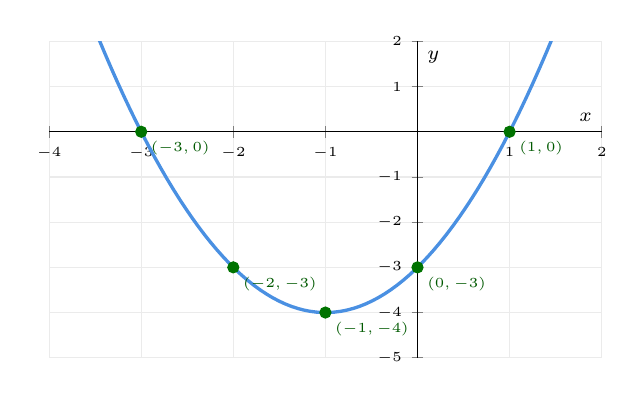
\begin{tikzpicture}\begin{axis}[width=8.6cm,height=5.6cm,axis lines=middle,xlabel={\scriptsize$x$},ylabel={\scriptsize$y$},grid=both,grid style={gray!16},xmin=-4,xmax=2,ymin=-5,ymax=2,xtick distance=1,ytick distance=1,tick label style={font=\tiny},axis line style={-}]
\addplot[exblue,very thick,domain=-4:2,samples=90]{x^2+2*x-3};\addplot[only marks,mark=*,mark size=2pt,green!45!black]coordinates{(-3,0)(-2,-3)(-1,-4)(0,-3)(1,0)};\node[font=\tiny,anchor=north west,green!35!black] at (axis cs:-3,0){$(-3,0)$};\node[font=\tiny,anchor=north west,green!35!black] at (axis cs:-2,-3){$(-2,-3)$};\node[font=\tiny,anchor=north west,green!35!black] at (axis cs:-1,-4){$(-1,-4)$};\node[font=\tiny,anchor=north west,green!35!black] at (axis cs:0,-3){$(0,-3)$};\node[font=\tiny,anchor=north west,green!35!black] at (axis cs:1,0){$(1,0)$};
\end{axis}\end{tikzpicture}\end{center}
\end{example}

\begin{example}{ex1}{Example 2 --- Linear, quadratic or neither?}
Use differences to classify each table.
\begin{center}\renewcommand{\arraystretch}{1.15}\setlength{\tabcolsep}{2pt}\begin{tabular}{r|>{\centering\arraybackslash}p{0.62cm}>{\centering\arraybackslash}p{0.62cm}>{\centering\arraybackslash}p{0.62cm}>{\centering\arraybackslash}p{0.62cm}>{\centering\arraybackslash}p{0.62cm}>{\centering\arraybackslash}p{0.62cm}>{\centering\arraybackslash}p{0.62cm}>{\centering\arraybackslash}p{0.62cm}>{\centering\arraybackslash}p{0.62cm}>{\centering\arraybackslash}p{0.62cm}}
$x$ & \multicolumn{2}{c}{\colorbox{iagreen}{\makebox[1.12cm]{\strut \color{white}\bfseries $0$}}} & \multicolumn{2}{c}{\colorbox{iagreen}{\makebox[1.12cm]{\strut \color{white}\bfseries $1$}}} & \multicolumn{2}{c}{\colorbox{iagreen}{\makebox[1.12cm]{\strut \color{white}\bfseries $2$}}} & \multicolumn{2}{c}{\colorbox{iagreen}{\makebox[1.12cm]{\strut \color{white}\bfseries $3$}}} & \multicolumn{2}{c}{\colorbox{iagreen}{\makebox[1.12cm]{\strut \color{white}\bfseries $4$}}} \\[2pt]
$A$ & \multicolumn{2}{c}{\colorbox{keybg}{\makebox[1.12cm]{\strut $-2$}}} & \multicolumn{2}{c}{\colorbox{keybg}{\makebox[1.12cm]{\strut $1$}}} & \multicolumn{2}{c}{\colorbox{keybg}{\makebox[1.12cm]{\strut $4$}}} & \multicolumn{2}{c}{\colorbox{keybg}{\makebox[1.12cm]{\strut $7$}}} & \multicolumn{2}{c}{\colorbox{keybg}{\makebox[1.12cm]{\strut $10$}}} \\[2pt]
\textcolor{exblue}{\scriptsize 1st diff} & & \multicolumn{2}{c}{\colorbox{exbg}{\makebox[1.12cm]{\strut \textcolor{exblue}{$+3$}}}} & \multicolumn{2}{c}{\colorbox{exbg}{\makebox[1.12cm]{\strut \textcolor{exblue}{$+3$}}}} & \multicolumn{2}{c}{\colorbox{exbg}{\makebox[1.12cm]{\strut \textcolor{exblue}{$+3$}}}} & \multicolumn{2}{c}{\colorbox{exbg}{\makebox[1.12cm]{\strut \textcolor{exblue}{$+3$}}}} & \\[2pt]
\textcolor{qorange}{\scriptsize 2nd diff} & & & \multicolumn{2}{c}{\colorbox{qbg}{\makebox[1.12cm]{\strut \textcolor{qorange!70!black}{$+0$}}}} & \multicolumn{2}{c}{\colorbox{qbg}{\makebox[1.12cm]{\strut \textcolor{qorange!70!black}{$+0$}}}} & \multicolumn{2}{c}{\colorbox{qbg}{\makebox[1.12cm]{\strut \textcolor{qorange!70!black}{$+0$}}}} & & \\
\end{tabular}\end{center}
\begin{center}\renewcommand{\arraystretch}{1.15}\setlength{\tabcolsep}{2pt}\begin{tabular}{r|>{\centering\arraybackslash}p{0.62cm}>{\centering\arraybackslash}p{0.62cm}>{\centering\arraybackslash}p{0.62cm}>{\centering\arraybackslash}p{0.62cm}>{\centering\arraybackslash}p{0.62cm}>{\centering\arraybackslash}p{0.62cm}>{\centering\arraybackslash}p{0.62cm}>{\centering\arraybackslash}p{0.62cm}>{\centering\arraybackslash}p{0.62cm}>{\centering\arraybackslash}p{0.62cm}}
$x$ & \multicolumn{2}{c}{\colorbox{iagreen}{\makebox[1.12cm]{\strut \color{white}\bfseries $0$}}} & \multicolumn{2}{c}{\colorbox{iagreen}{\makebox[1.12cm]{\strut \color{white}\bfseries $1$}}} & \multicolumn{2}{c}{\colorbox{iagreen}{\makebox[1.12cm]{\strut \color{white}\bfseries $2$}}} & \multicolumn{2}{c}{\colorbox{iagreen}{\makebox[1.12cm]{\strut \color{white}\bfseries $3$}}} & \multicolumn{2}{c}{\colorbox{iagreen}{\makebox[1.12cm]{\strut \color{white}\bfseries $4$}}} \\[2pt]
$B$ & \multicolumn{2}{c}{\colorbox{keybg}{\makebox[1.12cm]{\strut $0$}}} & \multicolumn{2}{c}{\colorbox{keybg}{\makebox[1.12cm]{\strut $-1$}}} & \multicolumn{2}{c}{\colorbox{keybg}{\makebox[1.12cm]{\strut $0$}}} & \multicolumn{2}{c}{\colorbox{keybg}{\makebox[1.12cm]{\strut $3$}}} & \multicolumn{2}{c}{\colorbox{keybg}{\makebox[1.12cm]{\strut $8$}}} \\[2pt]
\textcolor{exblue}{\scriptsize 1st diff} & & \multicolumn{2}{c}{\colorbox{exbg}{\makebox[1.12cm]{\strut \textcolor{exblue}{$-1$}}}} & \multicolumn{2}{c}{\colorbox{exbg}{\makebox[1.12cm]{\strut \textcolor{exblue}{$+1$}}}} & \multicolumn{2}{c}{\colorbox{exbg}{\makebox[1.12cm]{\strut \textcolor{exblue}{$+3$}}}} & \multicolumn{2}{c}{\colorbox{exbg}{\makebox[1.12cm]{\strut \textcolor{exblue}{$+5$}}}} & \\[2pt]
\textcolor{qorange}{\scriptsize 2nd diff} & & & \multicolumn{2}{c}{\colorbox{qbg}{\makebox[1.12cm]{\strut \textcolor{qorange!70!black}{$+2$}}}} & \multicolumn{2}{c}{\colorbox{qbg}{\makebox[1.12cm]{\strut \textcolor{qorange!70!black}{$+2$}}}} & \multicolumn{2}{c}{\colorbox{qbg}{\makebox[1.12cm]{\strut \textcolor{qorange!70!black}{$+2$}}}} & & \\
\end{tabular}\end{center}
\begin{center}\renewcommand{\arraystretch}{1.15}\setlength{\tabcolsep}{2pt}\begin{tabular}{r|>{\centering\arraybackslash}p{0.62cm}>{\centering\arraybackslash}p{0.62cm}>{\centering\arraybackslash}p{0.62cm}>{\centering\arraybackslash}p{0.62cm}>{\centering\arraybackslash}p{0.62cm}>{\centering\arraybackslash}p{0.62cm}>{\centering\arraybackslash}p{0.62cm}>{\centering\arraybackslash}p{0.62cm}>{\centering\arraybackslash}p{0.62cm}>{\centering\arraybackslash}p{0.62cm}}
$x$ & \multicolumn{2}{c}{\colorbox{iagreen}{\makebox[1.12cm]{\strut \color{white}\bfseries $0$}}} & \multicolumn{2}{c}{\colorbox{iagreen}{\makebox[1.12cm]{\strut \color{white}\bfseries $1$}}} & \multicolumn{2}{c}{\colorbox{iagreen}{\makebox[1.12cm]{\strut \color{white}\bfseries $2$}}} & \multicolumn{2}{c}{\colorbox{iagreen}{\makebox[1.12cm]{\strut \color{white}\bfseries $3$}}} & \multicolumn{2}{c}{\colorbox{iagreen}{\makebox[1.12cm]{\strut \color{white}\bfseries $4$}}} \\[2pt]
$C$ & \multicolumn{2}{c}{\colorbox{keybg}{\makebox[1.12cm]{\strut $1$}}} & \multicolumn{2}{c}{\colorbox{keybg}{\makebox[1.12cm]{\strut $3$}}} & \multicolumn{2}{c}{\colorbox{keybg}{\makebox[1.12cm]{\strut $9$}}} & \multicolumn{2}{c}{\colorbox{keybg}{\makebox[1.12cm]{\strut $27$}}} & \multicolumn{2}{c}{\colorbox{keybg}{\makebox[1.12cm]{\strut $81$}}} \\[2pt]
\textcolor{exblue}{\scriptsize 1st diff} & & \multicolumn{2}{c}{\colorbox{exbg}{\makebox[1.12cm]{\strut \textcolor{exblue}{$+2$}}}} & \multicolumn{2}{c}{\colorbox{exbg}{\makebox[1.12cm]{\strut \textcolor{exblue}{$+6$}}}} & \multicolumn{2}{c}{\colorbox{exbg}{\makebox[1.12cm]{\strut \textcolor{exblue}{$+18$}}}} & \multicolumn{2}{c}{\colorbox{exbg}{\makebox[1.12cm]{\strut \textcolor{exblue}{$+54$}}}} & \\[2pt]
\textcolor{qorange}{\scriptsize 2nd diff} & & & \multicolumn{2}{c}{\colorbox{qbg}{\makebox[1.12cm]{\strut \textcolor{qorange!70!black}{$+4$}}}} & \multicolumn{2}{c}{\colorbox{qbg}{\makebox[1.12cm]{\strut \textcolor{qorange!70!black}{$+12$}}}} & \multicolumn{2}{c}{\colorbox{qbg}{\makebox[1.12cm]{\strut \textcolor{qorange!70!black}{$+36$}}}} & & \\
\end{tabular}\end{center}
\soln \textbf{A:} 1st differences all $3$ --- linear. \textbf{B:} 1st differences $-1,1,3,5$ change, 2nd differences all $2$ --- quadratic. \textbf{C:} 1st differences $2,6,18,54$ and 2nd differences $4,12,36$ both keep changing --- neither.
\end{example}

\begin{example}{ex2}{Example 3 --- Is the point on the graph?}
The graph is $y=-x^2+4$. Is $(3,-5)$ on it? Is $(2,1)$?
\soln For $x=3$: $y=-9+4=-5$, so $(3,-5)$ \textbf{is} on the graph. For $x=2$: $y=-4+4=0\ne1$, so $(2,1)$ is \textbf{not} (the graph passes through $(2,0)$).
\begin{center}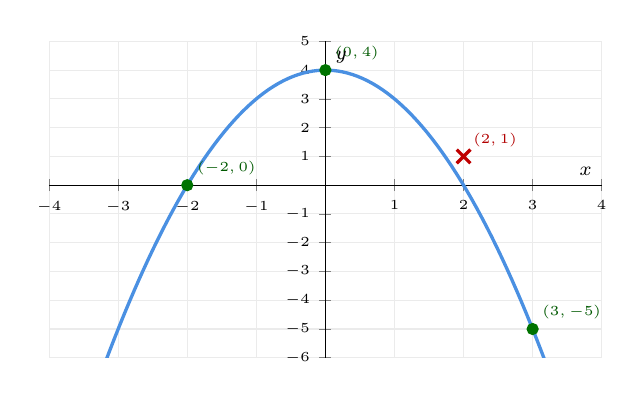
\begin{tikzpicture}\begin{axis}[width=8.6cm,height=5.6cm,axis lines=middle,xlabel={\scriptsize$x$},ylabel={\scriptsize$y$},grid=both,grid style={gray!16},xmin=-4,xmax=4,ymin=-6,ymax=5,xtick distance=1,ytick distance=1,tick label style={font=\tiny},axis line style={-}]
\addplot[exblue,very thick,domain=-3.2:3.2,samples=90]{-x^2+4};\addplot[only marks,mark=*,mark size=2pt,green!45!black]coordinates{(-2,0)(0,4)(3,-5)};\addplot[only marks,mark=x,mark size=3.5pt,very thick,red!75!black]coordinates{(2,1)};\node[font=\tiny,anchor=south west,green!35!black] at (axis cs:-2,0){$(-2,0)$};\node[font=\tiny,anchor=south west,green!35!black] at (axis cs:0,4){$(0,4)$};\node[font=\tiny,anchor=south west,green!35!black] at (axis cs:3,-5){$(3,-5)$};\node[font=\tiny,anchor=south west,red!70!black] at (axis cs:2,1){$(2,1)$};
\end{axis}\end{tikzpicture}\end{center}
\end{example}

\begin{example}{ex3}{Example 4 --- Find the missing value}
The relation is quadratic. Find the missing $y$-value.
\begin{center}\renewcommand{\arraystretch}{1.15}\setlength{\tabcolsep}{2pt}\begin{tabular}{r|>{\centering\arraybackslash}p{0.62cm}>{\centering\arraybackslash}p{0.62cm}>{\centering\arraybackslash}p{0.62cm}>{\centering\arraybackslash}p{0.62cm}>{\centering\arraybackslash}p{0.62cm}>{\centering\arraybackslash}p{0.62cm}>{\centering\arraybackslash}p{0.62cm}>{\centering\arraybackslash}p{0.62cm}>{\centering\arraybackslash}p{0.62cm}>{\centering\arraybackslash}p{0.62cm}}
$x$ & \multicolumn{2}{c}{\colorbox{iagreen}{\makebox[1.12cm]{\strut \color{white}\bfseries $0$}}} & \multicolumn{2}{c}{\colorbox{iagreen}{\makebox[1.12cm]{\strut \color{white}\bfseries $1$}}} & \multicolumn{2}{c}{\colorbox{iagreen}{\makebox[1.12cm]{\strut \color{white}\bfseries $2$}}} & \multicolumn{2}{c}{\colorbox{iagreen}{\makebox[1.12cm]{\strut \color{white}\bfseries $3$}}} & \multicolumn{2}{c}{\colorbox{iagreen}{\makebox[1.12cm]{\strut \color{white}\bfseries $4$}}} \\[2pt]
$y$ & \multicolumn{2}{c}{\colorbox{keybg}{\makebox[1.12cm]{\strut $1$}}} & \multicolumn{2}{c}{\colorbox{keybg}{\makebox[1.12cm]{\strut $2$}}} & \multicolumn{2}{c}{\fbox{\makebox[0.94cm]{\strut}}} & \multicolumn{2}{c}{\colorbox{keybg}{\makebox[1.12cm]{\strut $16$}}} & \multicolumn{2}{c}{\colorbox{keybg}{\makebox[1.12cm]{\strut $29$}}} \\[2pt]
\textcolor{exblue}{\scriptsize 1st diff} & & \multicolumn{2}{c}{\colorbox{exbg}{\makebox[1.12cm]{\strut \textcolor{exblue}{$+1$}}}} & \multicolumn{2}{c}{\colorbox{exbg}{\makebox[1.12cm]{\strut \textcolor{exblue}{$+5$}}}} & \multicolumn{2}{c}{\colorbox{exbg}{\makebox[1.12cm]{\strut \textcolor{exblue}{$+9$}}}} & \multicolumn{2}{c}{\colorbox{exbg}{\makebox[1.12cm]{\strut \textcolor{exblue}{$+13$}}}} & \\[2pt]
\textcolor{qorange}{\scriptsize 2nd diff} & & & \multicolumn{2}{c}{\colorbox{qbg}{\makebox[1.12cm]{\strut \textcolor{qorange!70!black}{$+4$}}}} & \multicolumn{2}{c}{\colorbox{qbg}{\makebox[1.12cm]{\strut \textcolor{qorange!70!black}{$+4$}}}} & \multicolumn{2}{c}{\colorbox{qbg}{\makebox[1.12cm]{\strut \textcolor{qorange!70!black}{$+4$}}}} & & \\
\end{tabular}\end{center}
\soln Known 1st differences: $1$ (first step) and $13$ (last step). If the 2nd difference is $d$, the last 1st difference is $1+3d=13$, so $d=4$. The 1st differences are $1,5,9,13$, so the missing value is $2+5=7$. Check: $7+9=16$ \checkmark.
\end{example}

\begin{example}{ex4}{Example 5 --- Find $a$, $b$ and $c$ from a table}
Find the equation $y=ax^2+bx+c$ from the table.
\begin{center}\renewcommand{\arraystretch}{1.15}\setlength{\tabcolsep}{2pt}\begin{tabular}{r|>{\centering\arraybackslash}p{0.62cm}>{\centering\arraybackslash}p{0.62cm}>{\centering\arraybackslash}p{0.62cm}>{\centering\arraybackslash}p{0.62cm}>{\centering\arraybackslash}p{0.62cm}>{\centering\arraybackslash}p{0.62cm}>{\centering\arraybackslash}p{0.62cm}>{\centering\arraybackslash}p{0.62cm}}
$x$ & \multicolumn{2}{c}{\colorbox{iagreen}{\makebox[1.12cm]{\strut \color{white}\bfseries $0$}}} & \multicolumn{2}{c}{\colorbox{iagreen}{\makebox[1.12cm]{\strut \color{white}\bfseries $1$}}} & \multicolumn{2}{c}{\colorbox{iagreen}{\makebox[1.12cm]{\strut \color{white}\bfseries $2$}}} & \multicolumn{2}{c}{\colorbox{iagreen}{\makebox[1.12cm]{\strut \color{white}\bfseries $3$}}} \\[2pt]
$y$ & \multicolumn{2}{c}{\colorbox{keybg}{\makebox[1.12cm]{\strut $5$}}} & \multicolumn{2}{c}{\colorbox{keybg}{\makebox[1.12cm]{\strut $6$}}} & \multicolumn{2}{c}{\colorbox{keybg}{\makebox[1.12cm]{\strut $11$}}} & \multicolumn{2}{c}{\colorbox{keybg}{\makebox[1.12cm]{\strut $20$}}} \\[2pt]
\textcolor{exblue}{\scriptsize 1st diff} & & \multicolumn{2}{c}{\colorbox{exbg}{\makebox[1.12cm]{\strut \textcolor{exblue}{$+1$}}}} & \multicolumn{2}{c}{\colorbox{exbg}{\makebox[1.12cm]{\strut \textcolor{exblue}{$+5$}}}} & \multicolumn{2}{c}{\colorbox{exbg}{\makebox[1.12cm]{\strut \textcolor{exblue}{$+9$}}}} & \\[2pt]
\textcolor{qorange}{\scriptsize 2nd diff} & & & \multicolumn{2}{c}{\colorbox{qbg}{\makebox[1.12cm]{\strut \textcolor{qorange!70!black}{$+4$}}}} & \multicolumn{2}{c}{\colorbox{qbg}{\makebox[1.12cm]{\strut \textcolor{qorange!70!black}{$+4$}}}} & & \\
\end{tabular}\end{center}
\soln 2nd difference $4=2a$, so $a=2$. $c=y(0)=5$. At $x=1$: $2+b+5=6$, so $b=-1$. $y=2x^2-x+5$. Check $x=3$: $18-3+5=20$ \checkmark.
\end{example}

\begin{example}{ex5}{Example 6 --- A parabola that opens down}
Use the table to find $a$, the direction of opening, and the maximum value.
\begin{center}\renewcommand{\arraystretch}{1.15}\setlength{\tabcolsep}{2pt}\begin{tabular}{r|>{\centering\arraybackslash}p{0.62cm}>{\centering\arraybackslash}p{0.62cm}>{\centering\arraybackslash}p{0.62cm}>{\centering\arraybackslash}p{0.62cm}>{\centering\arraybackslash}p{0.62cm}>{\centering\arraybackslash}p{0.62cm}>{\centering\arraybackslash}p{0.62cm}>{\centering\arraybackslash}p{0.62cm}>{\centering\arraybackslash}p{0.62cm}>{\centering\arraybackslash}p{0.62cm}}
$x$ & \multicolumn{2}{c}{\colorbox{iagreen}{\makebox[1.12cm]{\strut \color{white}\bfseries $0$}}} & \multicolumn{2}{c}{\colorbox{iagreen}{\makebox[1.12cm]{\strut \color{white}\bfseries $1$}}} & \multicolumn{2}{c}{\colorbox{iagreen}{\makebox[1.12cm]{\strut \color{white}\bfseries $2$}}} & \multicolumn{2}{c}{\colorbox{iagreen}{\makebox[1.12cm]{\strut \color{white}\bfseries $3$}}} & \multicolumn{2}{c}{\colorbox{iagreen}{\makebox[1.12cm]{\strut \color{white}\bfseries $4$}}} \\[2pt]
$y$ & \multicolumn{2}{c}{\colorbox{keybg}{\makebox[1.12cm]{\strut $-3$}}} & \multicolumn{2}{c}{\colorbox{keybg}{\makebox[1.12cm]{\strut $3$}}} & \multicolumn{2}{c}{\colorbox{keybg}{\makebox[1.12cm]{\strut $5$}}} & \multicolumn{2}{c}{\colorbox{keybg}{\makebox[1.12cm]{\strut $3$}}} & \multicolumn{2}{c}{\colorbox{keybg}{\makebox[1.12cm]{\strut $-3$}}} \\[2pt]
\textcolor{exblue}{\scriptsize 1st diff} & & \multicolumn{2}{c}{\colorbox{exbg}{\makebox[1.12cm]{\strut \textcolor{exblue}{$+6$}}}} & \multicolumn{2}{c}{\colorbox{exbg}{\makebox[1.12cm]{\strut \textcolor{exblue}{$+2$}}}} & \multicolumn{2}{c}{\colorbox{exbg}{\makebox[1.12cm]{\strut \textcolor{exblue}{$-2$}}}} & \multicolumn{2}{c}{\colorbox{exbg}{\makebox[1.12cm]{\strut \textcolor{exblue}{$-6$}}}} & \\[2pt]
\textcolor{qorange}{\scriptsize 2nd diff} & & & \multicolumn{2}{c}{\colorbox{qbg}{\makebox[1.12cm]{\strut \textcolor{qorange!70!black}{$-4$}}}} & \multicolumn{2}{c}{\colorbox{qbg}{\makebox[1.12cm]{\strut \textcolor{qorange!70!black}{$-4$}}}} & \multicolumn{2}{c}{\colorbox{qbg}{\makebox[1.12cm]{\strut \textcolor{qorange!70!black}{$-4$}}}} & & \\
\end{tabular}\end{center}
\soln 2nd difference $-4$, so $a=-2<0$: opens \textbf{down}. The values rise to $5$ at $x=2$, then fall: maximum value $5$, vertex $(2,5)$.
\begin{center}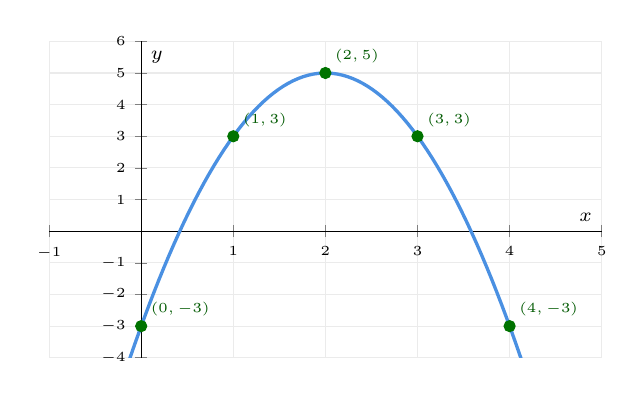
\begin{tikzpicture}\begin{axis}[width=8.6cm,height=5.6cm,axis lines=middle,xlabel={\scriptsize$x$},ylabel={\scriptsize$y$},grid=both,grid style={gray!16},xmin=-1,xmax=5,ymin=-4,ymax=6,xtick distance=1,ytick distance=1,tick label style={font=\tiny},axis line style={-}]
\addplot[exblue,very thick,domain=-0.4:4.4,samples=90]{-2*x^2+8*x-3};\addplot[only marks,mark=*,mark size=2pt,green!45!black]coordinates{(0,-3)(1,3)(2,5)(3,3)(4,-3)};\node[font=\tiny,anchor=south west,green!35!black] at (axis cs:0,-3){$(0,-3)$};\node[font=\tiny,anchor=south west,green!35!black] at (axis cs:1,3){$(1,3)$};\node[font=\tiny,anchor=south west,green!35!black] at (axis cs:2,5){$(2,5)$};\node[font=\tiny,anchor=south west,green!35!black] at (axis cs:3,3){$(3,3)$};\node[font=\tiny,anchor=south west,green!35!black] at (axis cs:4,-3){$(4,-3)$};
\end{axis}\end{tikzpicture}\end{center}
\end{example}

\begin{example}{ex6}{Example 7 --- Steps of 3}
The $x$-values go up by $3$. Find $a$ if $y=ax^2$.
\begin{center}\renewcommand{\arraystretch}{1.15}\setlength{\tabcolsep}{2pt}\begin{tabular}{r|>{\centering\arraybackslash}p{0.62cm}>{\centering\arraybackslash}p{0.62cm}>{\centering\arraybackslash}p{0.62cm}>{\centering\arraybackslash}p{0.62cm}>{\centering\arraybackslash}p{0.62cm}>{\centering\arraybackslash}p{0.62cm}>{\centering\arraybackslash}p{0.62cm}>{\centering\arraybackslash}p{0.62cm}}
$x$ & \multicolumn{2}{c}{\colorbox{iagreen}{\makebox[1.12cm]{\strut \color{white}\bfseries $0$}}} & \multicolumn{2}{c}{\colorbox{iagreen}{\makebox[1.12cm]{\strut \color{white}\bfseries $3$}}} & \multicolumn{2}{c}{\colorbox{iagreen}{\makebox[1.12cm]{\strut \color{white}\bfseries $6$}}} & \multicolumn{2}{c}{\colorbox{iagreen}{\makebox[1.12cm]{\strut \color{white}\bfseries $9$}}} \\[2pt]
$y$ & \multicolumn{2}{c}{\colorbox{keybg}{\makebox[1.12cm]{\strut $0$}}} & \multicolumn{2}{c}{\colorbox{keybg}{\makebox[1.12cm]{\strut $18$}}} & \multicolumn{2}{c}{\colorbox{keybg}{\makebox[1.12cm]{\strut $72$}}} & \multicolumn{2}{c}{\colorbox{keybg}{\makebox[1.12cm]{\strut $162$}}} \\[2pt]
\textcolor{exblue}{\scriptsize 1st diff} & & \multicolumn{2}{c}{\colorbox{exbg}{\makebox[1.12cm]{\strut \textcolor{exblue}{$+18$}}}} & \multicolumn{2}{c}{\colorbox{exbg}{\makebox[1.12cm]{\strut \textcolor{exblue}{$+54$}}}} & \multicolumn{2}{c}{\colorbox{exbg}{\makebox[1.12cm]{\strut \textcolor{exblue}{$+90$}}}} & \\[2pt]
\textcolor{qorange}{\scriptsize 2nd diff} & & & \multicolumn{2}{c}{\colorbox{qbg}{\makebox[1.12cm]{\strut \textcolor{qorange!70!black}{$+36$}}}} & \multicolumn{2}{c}{\colorbox{qbg}{\makebox[1.12cm]{\strut \textcolor{qorange!70!black}{$+36$}}}} & & \\
\end{tabular}\end{center}
\soln 1st differences $18,54,90$; 2nd differences $36,36$. With $h=3$: $2ah^2=18a=36$, so $a=2$. Check: $y(9)=2(81)=162$ \checkmark.
\end{example}

\begin{example}{ex7}{Example 8 --- Maximum area}
A fence of $40$ m encloses a rectangle of width $w$, so $A=w(20-w)$. Study the table.
\begin{center}\renewcommand{\arraystretch}{1.15}\setlength{\tabcolsep}{2pt}\begin{tabular}{r|>{\centering\arraybackslash}p{0.62cm}>{\centering\arraybackslash}p{0.62cm}>{\centering\arraybackslash}p{0.62cm}>{\centering\arraybackslash}p{0.62cm}>{\centering\arraybackslash}p{0.62cm}>{\centering\arraybackslash}p{0.62cm}>{\centering\arraybackslash}p{0.62cm}>{\centering\arraybackslash}p{0.62cm}>{\centering\arraybackslash}p{0.62cm}>{\centering\arraybackslash}p{0.62cm}}
$x$ & \multicolumn{2}{c}{\colorbox{iagreen}{\makebox[1.12cm]{\strut \color{white}\bfseries $0$}}} & \multicolumn{2}{c}{\colorbox{iagreen}{\makebox[1.12cm]{\strut \color{white}\bfseries $5$}}} & \multicolumn{2}{c}{\colorbox{iagreen}{\makebox[1.12cm]{\strut \color{white}\bfseries $10$}}} & \multicolumn{2}{c}{\colorbox{iagreen}{\makebox[1.12cm]{\strut \color{white}\bfseries $15$}}} & \multicolumn{2}{c}{\colorbox{iagreen}{\makebox[1.12cm]{\strut \color{white}\bfseries $20$}}} \\[2pt]
$A$ & \multicolumn{2}{c}{\colorbox{keybg}{\makebox[1.12cm]{\strut $0$}}} & \multicolumn{2}{c}{\colorbox{keybg}{\makebox[1.12cm]{\strut $75$}}} & \multicolumn{2}{c}{\colorbox{keybg}{\makebox[1.12cm]{\strut $100$}}} & \multicolumn{2}{c}{\colorbox{keybg}{\makebox[1.12cm]{\strut $75$}}} & \multicolumn{2}{c}{\colorbox{keybg}{\makebox[1.12cm]{\strut $0$}}} \\[2pt]
\textcolor{exblue}{\scriptsize 1st diff} & & \multicolumn{2}{c}{\colorbox{exbg}{\makebox[1.12cm]{\strut \textcolor{exblue}{$+75$}}}} & \multicolumn{2}{c}{\colorbox{exbg}{\makebox[1.12cm]{\strut \textcolor{exblue}{$+25$}}}} & \multicolumn{2}{c}{\colorbox{exbg}{\makebox[1.12cm]{\strut \textcolor{exblue}{$-25$}}}} & \multicolumn{2}{c}{\colorbox{exbg}{\makebox[1.12cm]{\strut \textcolor{exblue}{$-75$}}}} & \\[2pt]
\textcolor{qorange}{\scriptsize 2nd diff} & & & \multicolumn{2}{c}{\colorbox{qbg}{\makebox[1.12cm]{\strut \textcolor{qorange!70!black}{$-50$}}}} & \multicolumn{2}{c}{\colorbox{qbg}{\makebox[1.12cm]{\strut \textcolor{qorange!70!black}{$-50$}}}} & \multicolumn{2}{c}{\colorbox{qbg}{\makebox[1.12cm]{\strut \textcolor{qorange!70!black}{$-50$}}}} & & \\
\end{tabular}\end{center}
\soln 2nd differences $-50$; with $h=5$: $2ah^2=50a=-50$, so $a=-1$ (opens down). The largest area is $100\ \text{m}^2$ at $w=10$ m (a square $10$ by $10$).
\begin{center}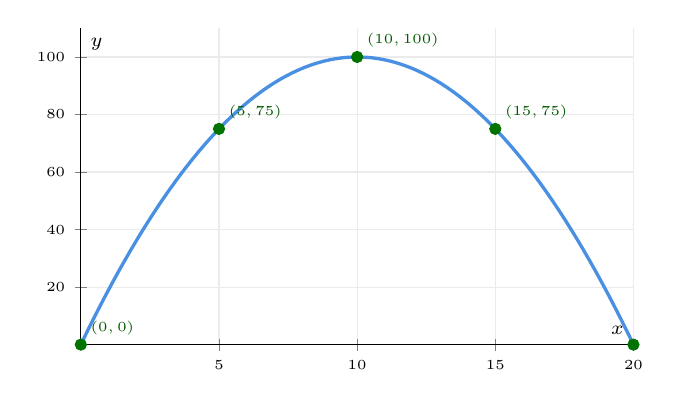
\begin{tikzpicture}\begin{axis}[width=8.6cm,height=5.6cm,axis lines=middle,xlabel={\scriptsize$x$},ylabel={\scriptsize$y$},grid=both,grid style={gray!16},xmin=0,xmax=20,ymin=0,ymax=110,xtick distance=5,ytick distance=20,tick label style={font=\tiny},axis line style={-}]
\addplot[exblue,very thick,domain=0:20,samples=90]{x*(20-x)};\addplot[only marks,mark=*,mark size=2pt,green!45!black]coordinates{(0,0)(5,75)(10,100)(15,75)(20,0)};\node[font=\tiny,anchor=south west,green!35!black] at (axis cs:0,0){$(0,0)$};\node[font=\tiny,anchor=south west,green!35!black] at (axis cs:5,75){$(5,75)$};\node[font=\tiny,anchor=south west,green!35!black] at (axis cs:10,100){$(10,100)$};\node[font=\tiny,anchor=south west,green!35!black] at (axis cs:15,75){$(15,75)$};\node[font=\tiny,anchor=south west,green!35!black] at (axis cs:20,0){$(20,0)$};
\end{axis}\end{tikzpicture}\end{center}
\end{example}

\begin{example}{ex8}{Example 9 --- Find the error}
A student says this table is quadratic. Find the mistake and the correct value.
\begin{center}\renewcommand{\arraystretch}{1.15}\setlength{\tabcolsep}{2pt}\begin{tabular}{r|>{\centering\arraybackslash}p{0.62cm}>{\centering\arraybackslash}p{0.62cm}>{\centering\arraybackslash}p{0.62cm}>{\centering\arraybackslash}p{0.62cm}>{\centering\arraybackslash}p{0.62cm}>{\centering\arraybackslash}p{0.62cm}>{\centering\arraybackslash}p{0.62cm}>{\centering\arraybackslash}p{0.62cm}>{\centering\arraybackslash}p{0.62cm}>{\centering\arraybackslash}p{0.62cm}}
$x$ & \multicolumn{2}{c}{\colorbox{iagreen}{\makebox[1.12cm]{\strut \color{white}\bfseries $0$}}} & \multicolumn{2}{c}{\colorbox{iagreen}{\makebox[1.12cm]{\strut \color{white}\bfseries $1$}}} & \multicolumn{2}{c}{\colorbox{iagreen}{\makebox[1.12cm]{\strut \color{white}\bfseries $2$}}} & \multicolumn{2}{c}{\colorbox{iagreen}{\makebox[1.12cm]{\strut \color{white}\bfseries $3$}}} & \multicolumn{2}{c}{\colorbox{iagreen}{\makebox[1.12cm]{\strut \color{white}\bfseries $4$}}} \\[2pt]
$y$ & \multicolumn{2}{c}{\colorbox{keybg}{\makebox[1.12cm]{\strut $2$}}} & \multicolumn{2}{c}{\colorbox{keybg}{\makebox[1.12cm]{\strut $3$}}} & \multicolumn{2}{c}{\colorbox{keybg}{\makebox[1.12cm]{\strut $6$}}} & \multicolumn{2}{c}{\colorbox{keybg}{\makebox[1.12cm]{\strut $11$}}} & \multicolumn{2}{c}{\colorbox{keybg}{\makebox[1.12cm]{\strut $20$}}} \\[2pt]
\textcolor{exblue}{\scriptsize 1st diff} & & \multicolumn{2}{c}{\colorbox{exbg}{\makebox[1.12cm]{\strut \textcolor{exblue}{$+1$}}}} & \multicolumn{2}{c}{\colorbox{exbg}{\makebox[1.12cm]{\strut \textcolor{exblue}{$+3$}}}} & \multicolumn{2}{c}{\colorbox{exbg}{\makebox[1.12cm]{\strut \textcolor{exblue}{$+5$}}}} & \multicolumn{2}{c}{\colorbox{exbg}{\makebox[1.12cm]{\strut \textcolor{exblue}{$+9$}}}} & \\[2pt]
\textcolor{qorange}{\scriptsize 2nd diff} & & & \multicolumn{2}{c}{\colorbox{qbg}{\makebox[1.12cm]{\strut \textcolor{qorange!70!black}{$+2$}}}} & \multicolumn{2}{c}{\colorbox{qbg}{\makebox[1.12cm]{\strut \textcolor{qorange!70!black}{$+2$}}}} & \multicolumn{2}{c}{\colorbox{qbg}{\makebox[1.12cm]{\strut \textcolor{qorange!70!black}{$+4$}}}} & & \\
\end{tabular}\end{center}
\soln 1st differences $1,3,5,9$; 2nd differences $2,2,4$ --- the last one breaks the pattern. The last 1st difference should be $7$, so the last value should be $11+7=18$, not $20$. Check on $y=x^2+2$: $y(4)=18$.
\begin{center}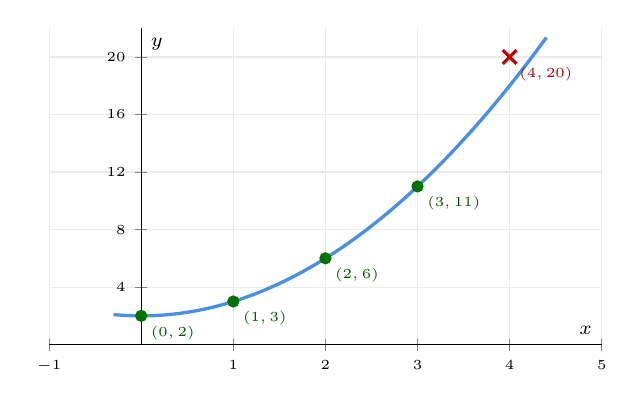
\begin{tikzpicture}\begin{axis}[width=8.6cm,height=5.6cm,axis lines=middle,xlabel={\scriptsize$x$},ylabel={\scriptsize$y$},grid=both,grid style={gray!16},xmin=-1,xmax=5,ymin=0,ymax=22,xtick distance=1,ytick distance=4,tick label style={font=\tiny},axis line style={-}]
\addplot[exblue,very thick,domain=-0.3:4.4,samples=90]{x^2+2};\addplot[only marks,mark=*,mark size=2pt,green!45!black]coordinates{(0,2)(1,3)(2,6)(3,11)};\addplot[only marks,mark=x,mark size=3.5pt,very thick,red!75!black]coordinates{(4,20)};\node[font=\tiny,anchor=north west,green!35!black] at (axis cs:0,2){$(0,2)$};\node[font=\tiny,anchor=north west,green!35!black] at (axis cs:1,3){$(1,3)$};\node[font=\tiny,anchor=north west,green!35!black] at (axis cs:2,6){$(2,6)$};\node[font=\tiny,anchor=north west,green!35!black] at (axis cs:3,11){$(3,11)$};\node[font=\tiny,anchor=north west,red!70!black] at (axis cs:4,20){$(4,20)$};
\end{axis}\end{tikzpicture}\end{center}
\end{example}

\clearpage
\sech{Your Turn --- Show Your Work}
For each question, show all steps clearly in the space provided.

\begin{qbox}{Question 1}
Complete the differences for each table and decide whether it is linear, quadratic or neither.
\begin{center}\renewcommand{\arraystretch}{1.15}\setlength{\tabcolsep}{2pt}\begin{tabular}{r|>{\centering\arraybackslash}p{0.62cm}>{\centering\arraybackslash}p{0.62cm}>{\centering\arraybackslash}p{0.62cm}>{\centering\arraybackslash}p{0.62cm}>{\centering\arraybackslash}p{0.62cm}>{\centering\arraybackslash}p{0.62cm}>{\centering\arraybackslash}p{0.62cm}>{\centering\arraybackslash}p{0.62cm}>{\centering\arraybackslash}p{0.62cm}>{\centering\arraybackslash}p{0.62cm}}
$x$ & \multicolumn{2}{c}{\colorbox{iagreen}{\makebox[1.12cm]{\strut \color{white}\bfseries $1$}}} & \multicolumn{2}{c}{\colorbox{iagreen}{\makebox[1.12cm]{\strut \color{white}\bfseries $2$}}} & \multicolumn{2}{c}{\colorbox{iagreen}{\makebox[1.12cm]{\strut \color{white}\bfseries $3$}}} & \multicolumn{2}{c}{\colorbox{iagreen}{\makebox[1.12cm]{\strut \color{white}\bfseries $4$}}} & \multicolumn{2}{c}{\colorbox{iagreen}{\makebox[1.12cm]{\strut \color{white}\bfseries $5$}}} \\[2pt]
$A$ & \multicolumn{2}{c}{\colorbox{keybg}{\makebox[1.12cm]{\strut $2$}}} & \multicolumn{2}{c}{\colorbox{keybg}{\makebox[1.12cm]{\strut $5$}}} & \multicolumn{2}{c}{\colorbox{keybg}{\makebox[1.12cm]{\strut $10$}}} & \multicolumn{2}{c}{\colorbox{keybg}{\makebox[1.12cm]{\strut $17$}}} & \multicolumn{2}{c}{\colorbox{keybg}{\makebox[1.12cm]{\strut $26$}}} \\[2pt]
\textcolor{exblue}{\scriptsize 1st diff} & & \multicolumn{2}{c}{\fbox{\makebox[0.94cm]{\strut}}} & \multicolumn{2}{c}{\fbox{\makebox[0.94cm]{\strut}}} & \multicolumn{2}{c}{\fbox{\makebox[0.94cm]{\strut}}} & \multicolumn{2}{c}{\fbox{\makebox[0.94cm]{\strut}}} & \\[2pt]
\textcolor{qorange}{\scriptsize 2nd diff} & & & \multicolumn{2}{c}{\fbox{\makebox[0.94cm]{\strut}}} & \multicolumn{2}{c}{\fbox{\makebox[0.94cm]{\strut}}} & \multicolumn{2}{c}{\fbox{\makebox[0.94cm]{\strut}}} & & \\
\end{tabular}\end{center}
\begin{center}\renewcommand{\arraystretch}{1.15}\setlength{\tabcolsep}{2pt}\begin{tabular}{r|>{\centering\arraybackslash}p{0.62cm}>{\centering\arraybackslash}p{0.62cm}>{\centering\arraybackslash}p{0.62cm}>{\centering\arraybackslash}p{0.62cm}>{\centering\arraybackslash}p{0.62cm}>{\centering\arraybackslash}p{0.62cm}>{\centering\arraybackslash}p{0.62cm}>{\centering\arraybackslash}p{0.62cm}>{\centering\arraybackslash}p{0.62cm}>{\centering\arraybackslash}p{0.62cm}}
$x$ & \multicolumn{2}{c}{\colorbox{iagreen}{\makebox[1.12cm]{\strut \color{white}\bfseries $0$}}} & \multicolumn{2}{c}{\colorbox{iagreen}{\makebox[1.12cm]{\strut \color{white}\bfseries $1$}}} & \multicolumn{2}{c}{\colorbox{iagreen}{\makebox[1.12cm]{\strut \color{white}\bfseries $2$}}} & \multicolumn{2}{c}{\colorbox{iagreen}{\makebox[1.12cm]{\strut \color{white}\bfseries $3$}}} & \multicolumn{2}{c}{\colorbox{iagreen}{\makebox[1.12cm]{\strut \color{white}\bfseries $4$}}} \\[2pt]
$B$ & \multicolumn{2}{c}{\colorbox{keybg}{\makebox[1.12cm]{\strut $-3$}}} & \multicolumn{2}{c}{\colorbox{keybg}{\makebox[1.12cm]{\strut $1$}}} & \multicolumn{2}{c}{\colorbox{keybg}{\makebox[1.12cm]{\strut $5$}}} & \multicolumn{2}{c}{\colorbox{keybg}{\makebox[1.12cm]{\strut $9$}}} & \multicolumn{2}{c}{\colorbox{keybg}{\makebox[1.12cm]{\strut $13$}}} \\[2pt]
\textcolor{exblue}{\scriptsize 1st diff} & & \multicolumn{2}{c}{\fbox{\makebox[0.94cm]{\strut}}} & \multicolumn{2}{c}{\fbox{\makebox[0.94cm]{\strut}}} & \multicolumn{2}{c}{\fbox{\makebox[0.94cm]{\strut}}} & \multicolumn{2}{c}{\fbox{\makebox[0.94cm]{\strut}}} & \\[2pt]
\textcolor{qorange}{\scriptsize 2nd diff} & & & \multicolumn{2}{c}{\fbox{\makebox[0.94cm]{\strut}}} & \multicolumn{2}{c}{\fbox{\makebox[0.94cm]{\strut}}} & \multicolumn{2}{c}{\fbox{\makebox[0.94cm]{\strut}}} & & \\
\end{tabular}\end{center}\workspace{1.0cm}
\end{qbox}

\begin{qbox}{Question 2}
Complete the table for $y=2x^2-3$, then fill in both difference rows.
\begin{center}\renewcommand{\arraystretch}{1.15}\setlength{\tabcolsep}{2pt}\begin{tabular}{r|>{\centering\arraybackslash}p{0.62cm}>{\centering\arraybackslash}p{0.62cm}>{\centering\arraybackslash}p{0.62cm}>{\centering\arraybackslash}p{0.62cm}>{\centering\arraybackslash}p{0.62cm}>{\centering\arraybackslash}p{0.62cm}>{\centering\arraybackslash}p{0.62cm}>{\centering\arraybackslash}p{0.62cm}>{\centering\arraybackslash}p{0.62cm}>{\centering\arraybackslash}p{0.62cm}}
$x$ & \multicolumn{2}{c}{\colorbox{iagreen}{\makebox[1.12cm]{\strut \color{white}\bfseries $-2$}}} & \multicolumn{2}{c}{\colorbox{iagreen}{\makebox[1.12cm]{\strut \color{white}\bfseries $-1$}}} & \multicolumn{2}{c}{\colorbox{iagreen}{\makebox[1.12cm]{\strut \color{white}\bfseries $0$}}} & \multicolumn{2}{c}{\colorbox{iagreen}{\makebox[1.12cm]{\strut \color{white}\bfseries $1$}}} & \multicolumn{2}{c}{\colorbox{iagreen}{\makebox[1.12cm]{\strut \color{white}\bfseries $2$}}} \\[2pt]
$y$ & \multicolumn{2}{c}{\fbox{\makebox[0.94cm]{\strut}}} & \multicolumn{2}{c}{\fbox{\makebox[0.94cm]{\strut}}} & \multicolumn{2}{c}{\fbox{\makebox[0.94cm]{\strut}}} & \multicolumn{2}{c}{\fbox{\makebox[0.94cm]{\strut}}} & \multicolumn{2}{c}{\fbox{\makebox[0.94cm]{\strut}}} \\[2pt]
\textcolor{exblue}{\scriptsize 1st diff} & & \multicolumn{2}{c}{\fbox{\makebox[0.94cm]{\strut}}} & \multicolumn{2}{c}{\fbox{\makebox[0.94cm]{\strut}}} & \multicolumn{2}{c}{\fbox{\makebox[0.94cm]{\strut}}} & \multicolumn{2}{c}{\fbox{\makebox[0.94cm]{\strut}}} & \\[2pt]
\textcolor{qorange}{\scriptsize 2nd diff} & & & \multicolumn{2}{c}{\fbox{\makebox[0.94cm]{\strut}}} & \multicolumn{2}{c}{\fbox{\makebox[0.94cm]{\strut}}} & \multicolumn{2}{c}{\fbox{\makebox[0.94cm]{\strut}}} & & \\
\end{tabular}\end{center}\workspace{1.2cm}
\end{qbox}

\begin{qbox}{Question 3}
This relation is quadratic. Find the missing value.
\begin{center}\renewcommand{\arraystretch}{1.15}\setlength{\tabcolsep}{2pt}\begin{tabular}{r|>{\centering\arraybackslash}p{0.62cm}>{\centering\arraybackslash}p{0.62cm}>{\centering\arraybackslash}p{0.62cm}>{\centering\arraybackslash}p{0.62cm}>{\centering\arraybackslash}p{0.62cm}>{\centering\arraybackslash}p{0.62cm}>{\centering\arraybackslash}p{0.62cm}>{\centering\arraybackslash}p{0.62cm}>{\centering\arraybackslash}p{0.62cm}>{\centering\arraybackslash}p{0.62cm}>{\centering\arraybackslash}p{0.62cm}>{\centering\arraybackslash}p{0.62cm}}
$x$ & \multicolumn{2}{c}{\colorbox{iagreen}{\makebox[1.12cm]{\strut \color{white}\bfseries $0$}}} & \multicolumn{2}{c}{\colorbox{iagreen}{\makebox[1.12cm]{\strut \color{white}\bfseries $1$}}} & \multicolumn{2}{c}{\colorbox{iagreen}{\makebox[1.12cm]{\strut \color{white}\bfseries $2$}}} & \multicolumn{2}{c}{\colorbox{iagreen}{\makebox[1.12cm]{\strut \color{white}\bfseries $3$}}} & \multicolumn{2}{c}{\colorbox{iagreen}{\makebox[1.12cm]{\strut \color{white}\bfseries $4$}}} & \multicolumn{2}{c}{\colorbox{iagreen}{\makebox[1.12cm]{\strut \color{white}\bfseries $5$}}} \\[2pt]
$y$ & \multicolumn{2}{c}{\colorbox{keybg}{\makebox[1.12cm]{\strut $4$}}} & \multicolumn{2}{c}{\colorbox{keybg}{\makebox[1.12cm]{\strut $2$}}} & \multicolumn{2}{c}{\colorbox{keybg}{\makebox[1.12cm]{\strut $2$}}} & \multicolumn{2}{c}{\fbox{\makebox[0.94cm]{\strut}}} & \multicolumn{2}{c}{\colorbox{keybg}{\makebox[1.12cm]{\strut $8$}}} & \multicolumn{2}{c}{\colorbox{keybg}{\makebox[1.12cm]{\strut $14$}}} \\[2pt]
\textcolor{exblue}{\scriptsize 1st diff} & & \multicolumn{2}{c}{\colorbox{exbg}{\makebox[1.12cm]{\strut \textcolor{exblue}{$-2$}}}} & \multicolumn{2}{c}{\colorbox{exbg}{\makebox[1.12cm]{\strut \textcolor{exblue}{$+0$}}}} & \multicolumn{2}{c}{\colorbox{exbg}{\makebox[1.12cm]{\strut \textcolor{exblue}{$+2$}}}} & \multicolumn{2}{c}{\colorbox{exbg}{\makebox[1.12cm]{\strut \textcolor{exblue}{$+4$}}}} & \multicolumn{2}{c}{\colorbox{exbg}{\makebox[1.12cm]{\strut \textcolor{exblue}{$+6$}}}} & \\[2pt]
\textcolor{qorange}{\scriptsize 2nd diff} & & & \multicolumn{2}{c}{\colorbox{qbg}{\makebox[1.12cm]{\strut \textcolor{qorange!70!black}{$+2$}}}} & \multicolumn{2}{c}{\colorbox{qbg}{\makebox[1.12cm]{\strut \textcolor{qorange!70!black}{$+2$}}}} & \multicolumn{2}{c}{\colorbox{qbg}{\makebox[1.12cm]{\strut \textcolor{qorange!70!black}{$+2$}}}} & \multicolumn{2}{c}{\colorbox{qbg}{\makebox[1.12cm]{\strut \textcolor{qorange!70!black}{$+2$}}}} & & \\
\end{tabular}\end{center}\workspace{2.2cm}
\end{qbox}

\begin{qbox}{Question 4}
The graph of $y=x^2-6x+7$ is shown. Which of $A(1,2)$, $B(2,-1)$, $C(4,-2)$, $D(5,3)$ lie on the graph? Correct the $y$-value of any point that does not.
\begin{center}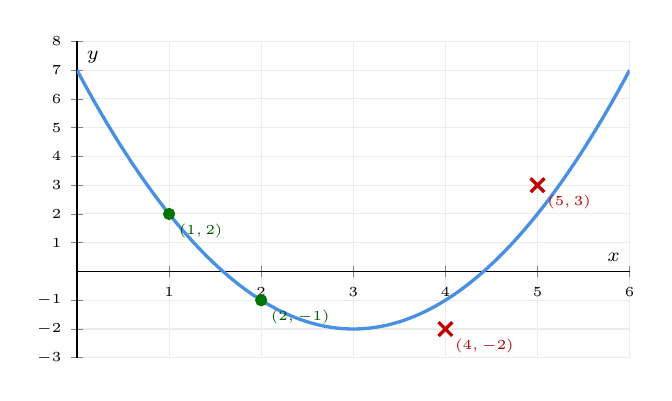
\begin{tikzpicture}\begin{axis}[width=8.6cm,height=5.6cm,axis lines=middle,xlabel={\scriptsize$x$},ylabel={\scriptsize$y$},grid=both,grid style={gray!16},xmin=0,xmax=6,ymin=-3,ymax=8,xtick distance=1,ytick distance=1,tick label style={font=\tiny},axis line style={-}]
\addplot[exblue,very thick,domain=0:6,samples=90]{x^2-6*x+7};\addplot[only marks,mark=*,mark size=2pt,green!45!black]coordinates{(1,2)(2,-1)};\addplot[only marks,mark=x,mark size=3.5pt,very thick,red!75!black]coordinates{(4,-2)(5,3)};\node[font=\tiny,anchor=north west,green!35!black] at (axis cs:1,2){$(1,2)$};\node[font=\tiny,anchor=north west,green!35!black] at (axis cs:2,-1){$(2,-1)$};\node[font=\tiny,anchor=north west,red!70!black] at (axis cs:4,-2){$(4,-2)$};\node[font=\tiny,anchor=north west,red!70!black] at (axis cs:5,3){$(5,3)$};
\end{axis}\end{tikzpicture}\end{center}\workspace{2.2cm}
\end{qbox}

\begin{qbox}{Question 5}
Find the equation $y=ax^2+bx+c$ of the relation.
\begin{center}\renewcommand{\arraystretch}{1.15}\setlength{\tabcolsep}{2pt}\begin{tabular}{r|>{\centering\arraybackslash}p{0.62cm}>{\centering\arraybackslash}p{0.62cm}>{\centering\arraybackslash}p{0.62cm}>{\centering\arraybackslash}p{0.62cm}>{\centering\arraybackslash}p{0.62cm}>{\centering\arraybackslash}p{0.62cm}>{\centering\arraybackslash}p{0.62cm}>{\centering\arraybackslash}p{0.62cm}}
$x$ & \multicolumn{2}{c}{\colorbox{iagreen}{\makebox[1.12cm]{\strut \color{white}\bfseries $0$}}} & \multicolumn{2}{c}{\colorbox{iagreen}{\makebox[1.12cm]{\strut \color{white}\bfseries $1$}}} & \multicolumn{2}{c}{\colorbox{iagreen}{\makebox[1.12cm]{\strut \color{white}\bfseries $2$}}} & \multicolumn{2}{c}{\colorbox{iagreen}{\makebox[1.12cm]{\strut \color{white}\bfseries $3$}}} \\[2pt]
$y$ & \multicolumn{2}{c}{\colorbox{keybg}{\makebox[1.12cm]{\strut $1$}}} & \multicolumn{2}{c}{\colorbox{keybg}{\makebox[1.12cm]{\strut $2$}}} & \multicolumn{2}{c}{\colorbox{keybg}{\makebox[1.12cm]{\strut $9$}}} & \multicolumn{2}{c}{\colorbox{keybg}{\makebox[1.12cm]{\strut $22$}}} \\[2pt]
\textcolor{exblue}{\scriptsize 1st diff} & & \multicolumn{2}{c}{\colorbox{exbg}{\makebox[1.12cm]{\strut \textcolor{exblue}{$+1$}}}} & \multicolumn{2}{c}{\colorbox{exbg}{\makebox[1.12cm]{\strut \textcolor{exblue}{$+7$}}}} & \multicolumn{2}{c}{\colorbox{exbg}{\makebox[1.12cm]{\strut \textcolor{exblue}{$+13$}}}} & \\[2pt]
\textcolor{qorange}{\scriptsize 2nd diff} & & & \multicolumn{2}{c}{\colorbox{qbg}{\makebox[1.12cm]{\strut \textcolor{qorange!70!black}{$+6$}}}} & \multicolumn{2}{c}{\colorbox{qbg}{\makebox[1.12cm]{\strut \textcolor{qorange!70!black}{$+6$}}}} & & \\
\end{tabular}\end{center}\workspace{2.8cm}
\end{qbox}

\begin{qbox}{Question 6}
Use the table to find $a$, say whether the parabola opens up or down, and give the vertex.
\begin{center}\renewcommand{\arraystretch}{1.15}\setlength{\tabcolsep}{2pt}\begin{tabular}{r|>{\centering\arraybackslash}p{0.62cm}>{\centering\arraybackslash}p{0.62cm}>{\centering\arraybackslash}p{0.62cm}>{\centering\arraybackslash}p{0.62cm}>{\centering\arraybackslash}p{0.62cm}>{\centering\arraybackslash}p{0.62cm}>{\centering\arraybackslash}p{0.62cm}>{\centering\arraybackslash}p{0.62cm}>{\centering\arraybackslash}p{0.62cm}>{\centering\arraybackslash}p{0.62cm}>{\centering\arraybackslash}p{0.62cm}>{\centering\arraybackslash}p{0.62cm}>{\centering\arraybackslash}p{0.62cm}>{\centering\arraybackslash}p{0.62cm}}
$x$ & \multicolumn{2}{c}{\colorbox{iagreen}{\makebox[1.12cm]{\strut \color{white}\bfseries $0$}}} & \multicolumn{2}{c}{\colorbox{iagreen}{\makebox[1.12cm]{\strut \color{white}\bfseries $1$}}} & \multicolumn{2}{c}{\colorbox{iagreen}{\makebox[1.12cm]{\strut \color{white}\bfseries $2$}}} & \multicolumn{2}{c}{\colorbox{iagreen}{\makebox[1.12cm]{\strut \color{white}\bfseries $3$}}} & \multicolumn{2}{c}{\colorbox{iagreen}{\makebox[1.12cm]{\strut \color{white}\bfseries $4$}}} & \multicolumn{2}{c}{\colorbox{iagreen}{\makebox[1.12cm]{\strut \color{white}\bfseries $5$}}} & \multicolumn{2}{c}{\colorbox{iagreen}{\makebox[1.12cm]{\strut \color{white}\bfseries $6$}}} \\[2pt]
$y$ & \multicolumn{2}{c}{\colorbox{keybg}{\makebox[1.12cm]{\strut $-4$}}} & \multicolumn{2}{c}{\colorbox{keybg}{\makebox[1.12cm]{\strut $1$}}} & \multicolumn{2}{c}{\colorbox{keybg}{\makebox[1.12cm]{\strut $4$}}} & \multicolumn{2}{c}{\colorbox{keybg}{\makebox[1.12cm]{\strut $5$}}} & \multicolumn{2}{c}{\colorbox{keybg}{\makebox[1.12cm]{\strut $4$}}} & \multicolumn{2}{c}{\colorbox{keybg}{\makebox[1.12cm]{\strut $1$}}} & \multicolumn{2}{c}{\colorbox{keybg}{\makebox[1.12cm]{\strut $-4$}}} \\[2pt]
\textcolor{exblue}{\scriptsize 1st diff} & & \multicolumn{2}{c}{\colorbox{exbg}{\makebox[1.12cm]{\strut \textcolor{exblue}{$+5$}}}} & \multicolumn{2}{c}{\colorbox{exbg}{\makebox[1.12cm]{\strut \textcolor{exblue}{$+3$}}}} & \multicolumn{2}{c}{\colorbox{exbg}{\makebox[1.12cm]{\strut \textcolor{exblue}{$+1$}}}} & \multicolumn{2}{c}{\colorbox{exbg}{\makebox[1.12cm]{\strut \textcolor{exblue}{$-1$}}}} & \multicolumn{2}{c}{\colorbox{exbg}{\makebox[1.12cm]{\strut \textcolor{exblue}{$-3$}}}} & \multicolumn{2}{c}{\colorbox{exbg}{\makebox[1.12cm]{\strut \textcolor{exblue}{$-5$}}}} & \\[2pt]
\textcolor{qorange}{\scriptsize 2nd diff} & & & \multicolumn{2}{c}{\colorbox{qbg}{\makebox[1.12cm]{\strut \textcolor{qorange!70!black}{$-2$}}}} & \multicolumn{2}{c}{\colorbox{qbg}{\makebox[1.12cm]{\strut \textcolor{qorange!70!black}{$-2$}}}} & \multicolumn{2}{c}{\colorbox{qbg}{\makebox[1.12cm]{\strut \textcolor{qorange!70!black}{$-2$}}}} & \multicolumn{2}{c}{\colorbox{qbg}{\makebox[1.12cm]{\strut \textcolor{qorange!70!black}{$-2$}}}} & \multicolumn{2}{c}{\colorbox{qbg}{\makebox[1.12cm]{\strut \textcolor{qorange!70!black}{$-2$}}}} & & \\
\end{tabular}\end{center}\workspace{2.8cm}
\end{qbox}

\begin{qbox}{Question 7}
The $x$-values go up by $2$. Find the equation $y=ax^2+bx+c$.
\begin{center}\renewcommand{\arraystretch}{1.15}\setlength{\tabcolsep}{2pt}\begin{tabular}{r|>{\centering\arraybackslash}p{0.62cm}>{\centering\arraybackslash}p{0.62cm}>{\centering\arraybackslash}p{0.62cm}>{\centering\arraybackslash}p{0.62cm}>{\centering\arraybackslash}p{0.62cm}>{\centering\arraybackslash}p{0.62cm}>{\centering\arraybackslash}p{0.62cm}>{\centering\arraybackslash}p{0.62cm}}
$x$ & \multicolumn{2}{c}{\colorbox{iagreen}{\makebox[1.12cm]{\strut \color{white}\bfseries $0$}}} & \multicolumn{2}{c}{\colorbox{iagreen}{\makebox[1.12cm]{\strut \color{white}\bfseries $2$}}} & \multicolumn{2}{c}{\colorbox{iagreen}{\makebox[1.12cm]{\strut \color{white}\bfseries $4$}}} & \multicolumn{2}{c}{\colorbox{iagreen}{\makebox[1.12cm]{\strut \color{white}\bfseries $6$}}} \\[2pt]
$y$ & \multicolumn{2}{c}{\colorbox{keybg}{\makebox[1.12cm]{\strut $1$}}} & \multicolumn{2}{c}{\colorbox{keybg}{\makebox[1.12cm]{\strut $5$}}} & \multicolumn{2}{c}{\colorbox{keybg}{\makebox[1.12cm]{\strut $17$}}} & \multicolumn{2}{c}{\colorbox{keybg}{\makebox[1.12cm]{\strut $37$}}} \\[2pt]
\textcolor{exblue}{\scriptsize 1st diff} & & \multicolumn{2}{c}{\colorbox{exbg}{\makebox[1.12cm]{\strut \textcolor{exblue}{$+4$}}}} & \multicolumn{2}{c}{\colorbox{exbg}{\makebox[1.12cm]{\strut \textcolor{exblue}{$+12$}}}} & \multicolumn{2}{c}{\colorbox{exbg}{\makebox[1.12cm]{\strut \textcolor{exblue}{$+20$}}}} & \\[2pt]
\textcolor{qorange}{\scriptsize 2nd diff} & & & \multicolumn{2}{c}{\colorbox{qbg}{\makebox[1.12cm]{\strut \textcolor{qorange!70!black}{$+8$}}}} & \multicolumn{2}{c}{\colorbox{qbg}{\makebox[1.12cm]{\strut \textcolor{qorange!70!black}{$+8$}}}} & & \\
\end{tabular}\end{center}\workspace{3.0cm}
\end{qbox}

\begin{qbox}{Question 8}
Read the points from the graph of $y=-x^2+2x+3$, complete the table and its differences, and state $a$.
\begin{center}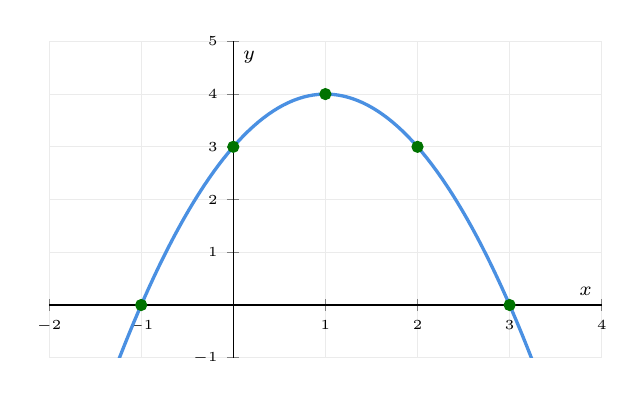
\begin{tikzpicture}\begin{axis}[width=8.6cm,height=5.6cm,axis lines=middle,xlabel={\scriptsize$x$},ylabel={\scriptsize$y$},grid=both,grid style={gray!16},xmin=-2,xmax=4,ymin=-1,ymax=5,xtick distance=1,ytick distance=1,tick label style={font=\tiny},axis line style={-}]
\addplot[exblue,very thick,domain=-1.4:3.4,samples=90]{-x^2+2*x+3};\addplot[only marks,mark=*,mark size=2pt,green!45!black]coordinates{(-1,0)(0,3)(1,4)(2,3)(3,0)};
\end{axis}\end{tikzpicture}\end{center}
\begin{center}\renewcommand{\arraystretch}{1.15}\setlength{\tabcolsep}{2pt}\begin{tabular}{r|>{\centering\arraybackslash}p{0.62cm}>{\centering\arraybackslash}p{0.62cm}>{\centering\arraybackslash}p{0.62cm}>{\centering\arraybackslash}p{0.62cm}>{\centering\arraybackslash}p{0.62cm}>{\centering\arraybackslash}p{0.62cm}>{\centering\arraybackslash}p{0.62cm}>{\centering\arraybackslash}p{0.62cm}>{\centering\arraybackslash}p{0.62cm}>{\centering\arraybackslash}p{0.62cm}}
$x$ & \multicolumn{2}{c}{\colorbox{iagreen}{\makebox[1.12cm]{\strut \color{white}\bfseries $-1$}}} & \multicolumn{2}{c}{\colorbox{iagreen}{\makebox[1.12cm]{\strut \color{white}\bfseries $0$}}} & \multicolumn{2}{c}{\colorbox{iagreen}{\makebox[1.12cm]{\strut \color{white}\bfseries $1$}}} & \multicolumn{2}{c}{\colorbox{iagreen}{\makebox[1.12cm]{\strut \color{white}\bfseries $2$}}} & \multicolumn{2}{c}{\colorbox{iagreen}{\makebox[1.12cm]{\strut \color{white}\bfseries $3$}}} \\[2pt]
$y$ & \multicolumn{2}{c}{\fbox{\makebox[0.94cm]{\strut}}} & \multicolumn{2}{c}{\fbox{\makebox[0.94cm]{\strut}}} & \multicolumn{2}{c}{\fbox{\makebox[0.94cm]{\strut}}} & \multicolumn{2}{c}{\fbox{\makebox[0.94cm]{\strut}}} & \multicolumn{2}{c}{\fbox{\makebox[0.94cm]{\strut}}} \\[2pt]
\textcolor{exblue}{\scriptsize 1st diff} & & \multicolumn{2}{c}{\fbox{\makebox[0.94cm]{\strut}}} & \multicolumn{2}{c}{\fbox{\makebox[0.94cm]{\strut}}} & \multicolumn{2}{c}{\fbox{\makebox[0.94cm]{\strut}}} & \multicolumn{2}{c}{\fbox{\makebox[0.94cm]{\strut}}} & \\[2pt]
\textcolor{qorange}{\scriptsize 2nd diff} & & & \multicolumn{2}{c}{\fbox{\makebox[0.94cm]{\strut}}} & \multicolumn{2}{c}{\fbox{\makebox[0.94cm]{\strut}}} & \multicolumn{2}{c}{\fbox{\makebox[0.94cm]{\strut}}} & & \\
\end{tabular}\end{center}\workspace{1.2cm}
\end{qbox}

\begin{qbox}{Question 9}
For $f(x)=x^2-5x+4$, find $f(-1)$ and $f(6)$. Is $(3,-2)$ on the graph of $f$? Show your substitution.\workspace{2.6cm}
\end{qbox}

\begin{qbox}{Question 10}
A ball's height is $h=-5t^2+30t$ (metres). Complete the table, find $a$ from the differences, the maximum height, and the time the ball is in the air.
\begin{center}\renewcommand{\arraystretch}{1.15}\setlength{\tabcolsep}{2pt}\begin{tabular}{r|>{\centering\arraybackslash}p{0.62cm}>{\centering\arraybackslash}p{0.62cm}>{\centering\arraybackslash}p{0.62cm}>{\centering\arraybackslash}p{0.62cm}>{\centering\arraybackslash}p{0.62cm}>{\centering\arraybackslash}p{0.62cm}>{\centering\arraybackslash}p{0.62cm}>{\centering\arraybackslash}p{0.62cm}>{\centering\arraybackslash}p{0.62cm}>{\centering\arraybackslash}p{0.62cm}>{\centering\arraybackslash}p{0.62cm}>{\centering\arraybackslash}p{0.62cm}>{\centering\arraybackslash}p{0.62cm}>{\centering\arraybackslash}p{0.62cm}}
$x$ & \multicolumn{2}{c}{\colorbox{iagreen}{\makebox[1.12cm]{\strut \color{white}\bfseries $0$}}} & \multicolumn{2}{c}{\colorbox{iagreen}{\makebox[1.12cm]{\strut \color{white}\bfseries $1$}}} & \multicolumn{2}{c}{\colorbox{iagreen}{\makebox[1.12cm]{\strut \color{white}\bfseries $2$}}} & \multicolumn{2}{c}{\colorbox{iagreen}{\makebox[1.12cm]{\strut \color{white}\bfseries $3$}}} & \multicolumn{2}{c}{\colorbox{iagreen}{\makebox[1.12cm]{\strut \color{white}\bfseries $4$}}} & \multicolumn{2}{c}{\colorbox{iagreen}{\makebox[1.12cm]{\strut \color{white}\bfseries $5$}}} & \multicolumn{2}{c}{\colorbox{iagreen}{\makebox[1.12cm]{\strut \color{white}\bfseries $6$}}} \\[2pt]
$h$ & \multicolumn{2}{c}{\fbox{\makebox[0.94cm]{\strut}}} & \multicolumn{2}{c}{\fbox{\makebox[0.94cm]{\strut}}} & \multicolumn{2}{c}{\fbox{\makebox[0.94cm]{\strut}}} & \multicolumn{2}{c}{\fbox{\makebox[0.94cm]{\strut}}} & \multicolumn{2}{c}{\fbox{\makebox[0.94cm]{\strut}}} & \multicolumn{2}{c}{\fbox{\makebox[0.94cm]{\strut}}} & \multicolumn{2}{c}{\fbox{\makebox[0.94cm]{\strut}}} \\[2pt]
\textcolor{exblue}{\scriptsize 1st diff} & & \multicolumn{2}{c}{\fbox{\makebox[0.94cm]{\strut}}} & \multicolumn{2}{c}{\fbox{\makebox[0.94cm]{\strut}}} & \multicolumn{2}{c}{\fbox{\makebox[0.94cm]{\strut}}} & \multicolumn{2}{c}{\fbox{\makebox[0.94cm]{\strut}}} & \multicolumn{2}{c}{\fbox{\makebox[0.94cm]{\strut}}} & \multicolumn{2}{c}{\fbox{\makebox[0.94cm]{\strut}}} & \\[2pt]
\textcolor{qorange}{\scriptsize 2nd diff} & & & \multicolumn{2}{c}{\fbox{\makebox[0.94cm]{\strut}}} & \multicolumn{2}{c}{\fbox{\makebox[0.94cm]{\strut}}} & \multicolumn{2}{c}{\fbox{\makebox[0.94cm]{\strut}}} & \multicolumn{2}{c}{\fbox{\makebox[0.94cm]{\strut}}} & \multicolumn{2}{c}{\fbox{\makebox[0.94cm]{\strut}}} & & \\
\end{tabular}\end{center}\workspace{2.4cm}
\end{qbox}

\begin{qbox}{Question 11}
One value in this table is wrong. Find it and correct it.
\begin{center}\renewcommand{\arraystretch}{1.15}\setlength{\tabcolsep}{2pt}\begin{tabular}{r|>{\centering\arraybackslash}p{0.62cm}>{\centering\arraybackslash}p{0.62cm}>{\centering\arraybackslash}p{0.62cm}>{\centering\arraybackslash}p{0.62cm}>{\centering\arraybackslash}p{0.62cm}>{\centering\arraybackslash}p{0.62cm}>{\centering\arraybackslash}p{0.62cm}>{\centering\arraybackslash}p{0.62cm}>{\centering\arraybackslash}p{0.62cm}>{\centering\arraybackslash}p{0.62cm}}
$x$ & \multicolumn{2}{c}{\colorbox{iagreen}{\makebox[1.12cm]{\strut \color{white}\bfseries $0$}}} & \multicolumn{2}{c}{\colorbox{iagreen}{\makebox[1.12cm]{\strut \color{white}\bfseries $1$}}} & \multicolumn{2}{c}{\colorbox{iagreen}{\makebox[1.12cm]{\strut \color{white}\bfseries $2$}}} & \multicolumn{2}{c}{\colorbox{iagreen}{\makebox[1.12cm]{\strut \color{white}\bfseries $3$}}} & \multicolumn{2}{c}{\colorbox{iagreen}{\makebox[1.12cm]{\strut \color{white}\bfseries $4$}}} \\[2pt]
$y$ & \multicolumn{2}{c}{\colorbox{keybg}{\makebox[1.12cm]{\strut $1$}}} & \multicolumn{2}{c}{\colorbox{keybg}{\makebox[1.12cm]{\strut $4$}}} & \multicolumn{2}{c}{\colorbox{keybg}{\makebox[1.12cm]{\strut $9$}}} & \multicolumn{2}{c}{\colorbox{keybg}{\makebox[1.12cm]{\strut $17$}}} & \multicolumn{2}{c}{\colorbox{keybg}{\makebox[1.12cm]{\strut $25$}}} \\[2pt]
\textcolor{exblue}{\scriptsize 1st diff} & & \multicolumn{2}{c}{\colorbox{exbg}{\makebox[1.12cm]{\strut \textcolor{exblue}{$+3$}}}} & \multicolumn{2}{c}{\colorbox{exbg}{\makebox[1.12cm]{\strut \textcolor{exblue}{$+5$}}}} & \multicolumn{2}{c}{\colorbox{exbg}{\makebox[1.12cm]{\strut \textcolor{exblue}{$+8$}}}} & \multicolumn{2}{c}{\colorbox{exbg}{\makebox[1.12cm]{\strut \textcolor{exblue}{$+8$}}}} & \\[2pt]
\textcolor{qorange}{\scriptsize 2nd diff} & & & \multicolumn{2}{c}{\colorbox{qbg}{\makebox[1.12cm]{\strut \textcolor{qorange!70!black}{$+2$}}}} & \multicolumn{2}{c}{\colorbox{qbg}{\makebox[1.12cm]{\strut \textcolor{qorange!70!black}{$+3$}}}} & \multicolumn{2}{c}{\colorbox{qbg}{\makebox[1.12cm]{\strut \textcolor{qorange!70!black}{$+0$}}}} & & \\
\end{tabular}\end{center}\workspace{2.2cm}
\end{qbox}

\begin{qbox}{Question 12}
Show that for $y=ax^2+bx+c$ and $x=0,1,2$, the second difference is $2a$.\workspace{3.2cm}
\end{qbox}

\begin{qbox}{Question 13 --- Challenge}
A quadratic relation passes through $(0,-5)$, $(1,-2)$ and $(2,5)$. Find $y$ when $x=10$, and say whether $(3,16)$ is on the graph.\workspace{3.4cm}
\end{qbox}

\clearpage
\sech{Question Recap \& Answer Key}

\begin{recapbox}
\begin{multicols}{2}
\small
\begin{enumerate}[leftmargin=*,itemsep=3pt]
  \item Complete the differences for each table and decide whether it is linear, quadratic or neither.
\begin{center}\renewcommand{\arraystretch}{1.15}\setlength{\tabcolsep}{2pt}\begin{tabular}{r|>{\centering\arraybackslash}p{0.62cm}>{\centering\arraybackslash}p{0.62cm}>{\centering\arraybackslash}p{0.62cm}>{\centering\arraybackslash}p{0.62cm}>{\centering\arraybackslash}p{0.62cm}>{\centering\arraybackslash}p{0.62cm}>{\centering\arraybackslash}p{0.62cm}>{\centering\arraybackslash}p{0.62cm}>{\centering\arraybackslash}p{0.62cm}>{\centering\arraybackslash}p{0.62cm}}
$x$ & \multicolumn{2}{c}{\colorbox{iagreen}{\makebox[1.12cm]{\strut \color{white}\bfseries $1$}}} & \multicolumn{2}{c}{\colorbox{iagreen}{\makebox[1.12cm]{\strut \color{white}\bfseries $2$}}} & \multicolumn{2}{c}{\colorbox{iagreen}{\makebox[1.12cm]{\strut \color{white}\bfseries $3$}}} & \multicolumn{2}{c}{\colorbox{iagreen}{\makebox[1.12cm]{\strut \color{white}\bfseries $4$}}} & \multicolumn{2}{c}{\colorbox{iagreen}{\makebox[1.12cm]{\strut \color{white}\bfseries $5$}}} \\[2pt]
$A$ & \multicolumn{2}{c}{\colorbox{keybg}{\makebox[1.12cm]{\strut $2$}}} & \multicolumn{2}{c}{\colorbox{keybg}{\makebox[1.12cm]{\strut $5$}}} & \multicolumn{2}{c}{\colorbox{keybg}{\makebox[1.12cm]{\strut $10$}}} & \multicolumn{2}{c}{\colorbox{keybg}{\makebox[1.12cm]{\strut $17$}}} & \multicolumn{2}{c}{\colorbox{keybg}{\makebox[1.12cm]{\strut $26$}}} \\[2pt]
\textcolor{exblue}{\scriptsize 1st diff} & & \multicolumn{2}{c}{\fbox{\makebox[0.94cm]{\strut}}} & \multicolumn{2}{c}{\fbox{\makebox[0.94cm]{\strut}}} & \multicolumn{2}{c}{\fbox{\makebox[0.94cm]{\strut}}} & \multicolumn{2}{c}{\fbox{\makebox[0.94cm]{\strut}}} & \\[2pt]
\textcolor{qorange}{\scriptsize 2nd diff} & & & \multicolumn{2}{c}{\fbox{\makebox[0.94cm]{\strut}}} & \multicolumn{2}{c}{\fbox{\makebox[0.94cm]{\strut}}} & \multicolumn{2}{c}{\fbox{\makebox[0.94cm]{\strut}}} & & \\
\end{tabular}\end{center}
\begin{center}\renewcommand{\arraystretch}{1.15}\setlength{\tabcolsep}{2pt}\begin{tabular}{r|>{\centering\arraybackslash}p{0.62cm}>{\centering\arraybackslash}p{0.62cm}>{\centering\arraybackslash}p{0.62cm}>{\centering\arraybackslash}p{0.62cm}>{\centering\arraybackslash}p{0.62cm}>{\centering\arraybackslash}p{0.62cm}>{\centering\arraybackslash}p{0.62cm}>{\centering\arraybackslash}p{0.62cm}>{\centering\arraybackslash}p{0.62cm}>{\centering\arraybackslash}p{0.62cm}}
$x$ & \multicolumn{2}{c}{\colorbox{iagreen}{\makebox[1.12cm]{\strut \color{white}\bfseries $0$}}} & \multicolumn{2}{c}{\colorbox{iagreen}{\makebox[1.12cm]{\strut \color{white}\bfseries $1$}}} & \multicolumn{2}{c}{\colorbox{iagreen}{\makebox[1.12cm]{\strut \color{white}\bfseries $2$}}} & \multicolumn{2}{c}{\colorbox{iagreen}{\makebox[1.12cm]{\strut \color{white}\bfseries $3$}}} & \multicolumn{2}{c}{\colorbox{iagreen}{\makebox[1.12cm]{\strut \color{white}\bfseries $4$}}} \\[2pt]
$B$ & \multicolumn{2}{c}{\colorbox{keybg}{\makebox[1.12cm]{\strut $-3$}}} & \multicolumn{2}{c}{\colorbox{keybg}{\makebox[1.12cm]{\strut $1$}}} & \multicolumn{2}{c}{\colorbox{keybg}{\makebox[1.12cm]{\strut $5$}}} & \multicolumn{2}{c}{\colorbox{keybg}{\makebox[1.12cm]{\strut $9$}}} & \multicolumn{2}{c}{\colorbox{keybg}{\makebox[1.12cm]{\strut $13$}}} \\[2pt]
\textcolor{exblue}{\scriptsize 1st diff} & & \multicolumn{2}{c}{\fbox{\makebox[0.94cm]{\strut}}} & \multicolumn{2}{c}{\fbox{\makebox[0.94cm]{\strut}}} & \multicolumn{2}{c}{\fbox{\makebox[0.94cm]{\strut}}} & \multicolumn{2}{c}{\fbox{\makebox[0.94cm]{\strut}}} & \\[2pt]
\textcolor{qorange}{\scriptsize 2nd diff} & & & \multicolumn{2}{c}{\fbox{\makebox[0.94cm]{\strut}}} & \multicolumn{2}{c}{\fbox{\makebox[0.94cm]{\strut}}} & \multicolumn{2}{c}{\fbox{\makebox[0.94cm]{\strut}}} & & \\
\end{tabular}\end{center}
  \item Complete the table for $y=2x^2-3$, then fill in both difference rows.
\begin{center}\renewcommand{\arraystretch}{1.15}\setlength{\tabcolsep}{2pt}\begin{tabular}{r|>{\centering\arraybackslash}p{0.62cm}>{\centering\arraybackslash}p{0.62cm}>{\centering\arraybackslash}p{0.62cm}>{\centering\arraybackslash}p{0.62cm}>{\centering\arraybackslash}p{0.62cm}>{\centering\arraybackslash}p{0.62cm}>{\centering\arraybackslash}p{0.62cm}>{\centering\arraybackslash}p{0.62cm}>{\centering\arraybackslash}p{0.62cm}>{\centering\arraybackslash}p{0.62cm}}
$x$ & \multicolumn{2}{c}{\colorbox{iagreen}{\makebox[1.12cm]{\strut \color{white}\bfseries $-2$}}} & \multicolumn{2}{c}{\colorbox{iagreen}{\makebox[1.12cm]{\strut \color{white}\bfseries $-1$}}} & \multicolumn{2}{c}{\colorbox{iagreen}{\makebox[1.12cm]{\strut \color{white}\bfseries $0$}}} & \multicolumn{2}{c}{\colorbox{iagreen}{\makebox[1.12cm]{\strut \color{white}\bfseries $1$}}} & \multicolumn{2}{c}{\colorbox{iagreen}{\makebox[1.12cm]{\strut \color{white}\bfseries $2$}}} \\[2pt]
$y$ & \multicolumn{2}{c}{\fbox{\makebox[0.94cm]{\strut}}} & \multicolumn{2}{c}{\fbox{\makebox[0.94cm]{\strut}}} & \multicolumn{2}{c}{\fbox{\makebox[0.94cm]{\strut}}} & \multicolumn{2}{c}{\fbox{\makebox[0.94cm]{\strut}}} & \multicolumn{2}{c}{\fbox{\makebox[0.94cm]{\strut}}} \\[2pt]
\textcolor{exblue}{\scriptsize 1st diff} & & \multicolumn{2}{c}{\fbox{\makebox[0.94cm]{\strut}}} & \multicolumn{2}{c}{\fbox{\makebox[0.94cm]{\strut}}} & \multicolumn{2}{c}{\fbox{\makebox[0.94cm]{\strut}}} & \multicolumn{2}{c}{\fbox{\makebox[0.94cm]{\strut}}} & \\[2pt]
\textcolor{qorange}{\scriptsize 2nd diff} & & & \multicolumn{2}{c}{\fbox{\makebox[0.94cm]{\strut}}} & \multicolumn{2}{c}{\fbox{\makebox[0.94cm]{\strut}}} & \multicolumn{2}{c}{\fbox{\makebox[0.94cm]{\strut}}} & & \\
\end{tabular}\end{center}
  \item This relation is quadratic. Find the missing value.
\begin{center}\renewcommand{\arraystretch}{1.15}\setlength{\tabcolsep}{2pt}\begin{tabular}{r|>{\centering\arraybackslash}p{0.62cm}>{\centering\arraybackslash}p{0.62cm}>{\centering\arraybackslash}p{0.62cm}>{\centering\arraybackslash}p{0.62cm}>{\centering\arraybackslash}p{0.62cm}>{\centering\arraybackslash}p{0.62cm}>{\centering\arraybackslash}p{0.62cm}>{\centering\arraybackslash}p{0.62cm}>{\centering\arraybackslash}p{0.62cm}>{\centering\arraybackslash}p{0.62cm}>{\centering\arraybackslash}p{0.62cm}>{\centering\arraybackslash}p{0.62cm}}
$x$ & \multicolumn{2}{c}{\colorbox{iagreen}{\makebox[1.12cm]{\strut \color{white}\bfseries $0$}}} & \multicolumn{2}{c}{\colorbox{iagreen}{\makebox[1.12cm]{\strut \color{white}\bfseries $1$}}} & \multicolumn{2}{c}{\colorbox{iagreen}{\makebox[1.12cm]{\strut \color{white}\bfseries $2$}}} & \multicolumn{2}{c}{\colorbox{iagreen}{\makebox[1.12cm]{\strut \color{white}\bfseries $3$}}} & \multicolumn{2}{c}{\colorbox{iagreen}{\makebox[1.12cm]{\strut \color{white}\bfseries $4$}}} & \multicolumn{2}{c}{\colorbox{iagreen}{\makebox[1.12cm]{\strut \color{white}\bfseries $5$}}} \\[2pt]
$y$ & \multicolumn{2}{c}{\colorbox{keybg}{\makebox[1.12cm]{\strut $4$}}} & \multicolumn{2}{c}{\colorbox{keybg}{\makebox[1.12cm]{\strut $2$}}} & \multicolumn{2}{c}{\colorbox{keybg}{\makebox[1.12cm]{\strut $2$}}} & \multicolumn{2}{c}{\fbox{\makebox[0.94cm]{\strut}}} & \multicolumn{2}{c}{\colorbox{keybg}{\makebox[1.12cm]{\strut $8$}}} & \multicolumn{2}{c}{\colorbox{keybg}{\makebox[1.12cm]{\strut $14$}}} \\[2pt]
\textcolor{exblue}{\scriptsize 1st diff} & & \multicolumn{2}{c}{\colorbox{exbg}{\makebox[1.12cm]{\strut \textcolor{exblue}{$-2$}}}} & \multicolumn{2}{c}{\colorbox{exbg}{\makebox[1.12cm]{\strut \textcolor{exblue}{$+0$}}}} & \multicolumn{2}{c}{\colorbox{exbg}{\makebox[1.12cm]{\strut \textcolor{exblue}{$+2$}}}} & \multicolumn{2}{c}{\colorbox{exbg}{\makebox[1.12cm]{\strut \textcolor{exblue}{$+4$}}}} & \multicolumn{2}{c}{\colorbox{exbg}{\makebox[1.12cm]{\strut \textcolor{exblue}{$+6$}}}} & \\[2pt]
\textcolor{qorange}{\scriptsize 2nd diff} & & & \multicolumn{2}{c}{\colorbox{qbg}{\makebox[1.12cm]{\strut \textcolor{qorange!70!black}{$+2$}}}} & \multicolumn{2}{c}{\colorbox{qbg}{\makebox[1.12cm]{\strut \textcolor{qorange!70!black}{$+2$}}}} & \multicolumn{2}{c}{\colorbox{qbg}{\makebox[1.12cm]{\strut \textcolor{qorange!70!black}{$+2$}}}} & \multicolumn{2}{c}{\colorbox{qbg}{\makebox[1.12cm]{\strut \textcolor{qorange!70!black}{$+2$}}}} & & \\
\end{tabular}\end{center}
  \item The graph of $y=x^2-6x+7$ is shown. Which of $A(1,2)$, $B(2,-1)$, $C(4,-2)$, $D(5,3)$ lie on the graph? Correct the $y$-value of any point that does not.
\begin{center}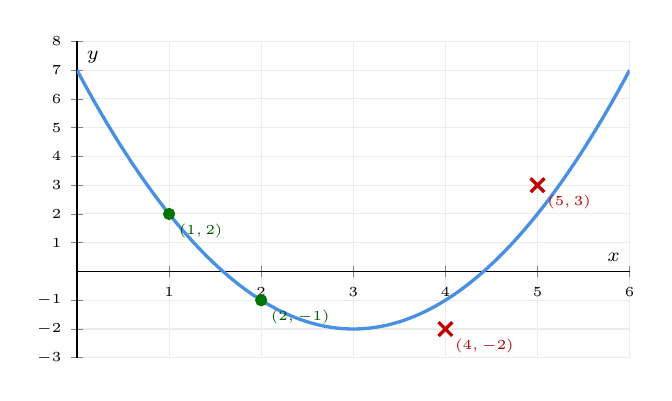
\begin{tikzpicture}\begin{axis}[width=8.6cm,height=5.6cm,axis lines=middle,xlabel={\scriptsize$x$},ylabel={\scriptsize$y$},grid=both,grid style={gray!16},xmin=0,xmax=6,ymin=-3,ymax=8,xtick distance=1,ytick distance=1,tick label style={font=\tiny},axis line style={-}]
\addplot[exblue,very thick,domain=0:6,samples=90]{x^2-6*x+7};\addplot[only marks,mark=*,mark size=2pt,green!45!black]coordinates{(1,2)(2,-1)};\addplot[only marks,mark=x,mark size=3.5pt,very thick,red!75!black]coordinates{(4,-2)(5,3)};\node[font=\tiny,anchor=north west,green!35!black] at (axis cs:1,2){$(1,2)$};\node[font=\tiny,anchor=north west,green!35!black] at (axis cs:2,-1){$(2,-1)$};\node[font=\tiny,anchor=north west,red!70!black] at (axis cs:4,-2){$(4,-2)$};\node[font=\tiny,anchor=north west,red!70!black] at (axis cs:5,3){$(5,3)$};
\end{axis}\end{tikzpicture}\end{center}
  \item Find the equation $y=ax^2+bx+c$ of the relation.
\begin{center}\renewcommand{\arraystretch}{1.15}\setlength{\tabcolsep}{2pt}\begin{tabular}{r|>{\centering\arraybackslash}p{0.62cm}>{\centering\arraybackslash}p{0.62cm}>{\centering\arraybackslash}p{0.62cm}>{\centering\arraybackslash}p{0.62cm}>{\centering\arraybackslash}p{0.62cm}>{\centering\arraybackslash}p{0.62cm}>{\centering\arraybackslash}p{0.62cm}>{\centering\arraybackslash}p{0.62cm}}
$x$ & \multicolumn{2}{c}{\colorbox{iagreen}{\makebox[1.12cm]{\strut \color{white}\bfseries $0$}}} & \multicolumn{2}{c}{\colorbox{iagreen}{\makebox[1.12cm]{\strut \color{white}\bfseries $1$}}} & \multicolumn{2}{c}{\colorbox{iagreen}{\makebox[1.12cm]{\strut \color{white}\bfseries $2$}}} & \multicolumn{2}{c}{\colorbox{iagreen}{\makebox[1.12cm]{\strut \color{white}\bfseries $3$}}} \\[2pt]
$y$ & \multicolumn{2}{c}{\colorbox{keybg}{\makebox[1.12cm]{\strut $1$}}} & \multicolumn{2}{c}{\colorbox{keybg}{\makebox[1.12cm]{\strut $2$}}} & \multicolumn{2}{c}{\colorbox{keybg}{\makebox[1.12cm]{\strut $9$}}} & \multicolumn{2}{c}{\colorbox{keybg}{\makebox[1.12cm]{\strut $22$}}} \\[2pt]
\textcolor{exblue}{\scriptsize 1st diff} & & \multicolumn{2}{c}{\colorbox{exbg}{\makebox[1.12cm]{\strut \textcolor{exblue}{$+1$}}}} & \multicolumn{2}{c}{\colorbox{exbg}{\makebox[1.12cm]{\strut \textcolor{exblue}{$+7$}}}} & \multicolumn{2}{c}{\colorbox{exbg}{\makebox[1.12cm]{\strut \textcolor{exblue}{$+13$}}}} & \\[2pt]
\textcolor{qorange}{\scriptsize 2nd diff} & & & \multicolumn{2}{c}{\colorbox{qbg}{\makebox[1.12cm]{\strut \textcolor{qorange!70!black}{$+6$}}}} & \multicolumn{2}{c}{\colorbox{qbg}{\makebox[1.12cm]{\strut \textcolor{qorange!70!black}{$+6$}}}} & & \\
\end{tabular}\end{center}
  \item Use the table to find $a$, say whether the parabola opens up or down, and give the vertex.
\begin{center}\renewcommand{\arraystretch}{1.15}\setlength{\tabcolsep}{2pt}\begin{tabular}{r|>{\centering\arraybackslash}p{0.62cm}>{\centering\arraybackslash}p{0.62cm}>{\centering\arraybackslash}p{0.62cm}>{\centering\arraybackslash}p{0.62cm}>{\centering\arraybackslash}p{0.62cm}>{\centering\arraybackslash}p{0.62cm}>{\centering\arraybackslash}p{0.62cm}>{\centering\arraybackslash}p{0.62cm}>{\centering\arraybackslash}p{0.62cm}>{\centering\arraybackslash}p{0.62cm}>{\centering\arraybackslash}p{0.62cm}>{\centering\arraybackslash}p{0.62cm}>{\centering\arraybackslash}p{0.62cm}>{\centering\arraybackslash}p{0.62cm}}
$x$ & \multicolumn{2}{c}{\colorbox{iagreen}{\makebox[1.12cm]{\strut \color{white}\bfseries $0$}}} & \multicolumn{2}{c}{\colorbox{iagreen}{\makebox[1.12cm]{\strut \color{white}\bfseries $1$}}} & \multicolumn{2}{c}{\colorbox{iagreen}{\makebox[1.12cm]{\strut \color{white}\bfseries $2$}}} & \multicolumn{2}{c}{\colorbox{iagreen}{\makebox[1.12cm]{\strut \color{white}\bfseries $3$}}} & \multicolumn{2}{c}{\colorbox{iagreen}{\makebox[1.12cm]{\strut \color{white}\bfseries $4$}}} & \multicolumn{2}{c}{\colorbox{iagreen}{\makebox[1.12cm]{\strut \color{white}\bfseries $5$}}} & \multicolumn{2}{c}{\colorbox{iagreen}{\makebox[1.12cm]{\strut \color{white}\bfseries $6$}}} \\[2pt]
$y$ & \multicolumn{2}{c}{\colorbox{keybg}{\makebox[1.12cm]{\strut $-4$}}} & \multicolumn{2}{c}{\colorbox{keybg}{\makebox[1.12cm]{\strut $1$}}} & \multicolumn{2}{c}{\colorbox{keybg}{\makebox[1.12cm]{\strut $4$}}} & \multicolumn{2}{c}{\colorbox{keybg}{\makebox[1.12cm]{\strut $5$}}} & \multicolumn{2}{c}{\colorbox{keybg}{\makebox[1.12cm]{\strut $4$}}} & \multicolumn{2}{c}{\colorbox{keybg}{\makebox[1.12cm]{\strut $1$}}} & \multicolumn{2}{c}{\colorbox{keybg}{\makebox[1.12cm]{\strut $-4$}}} \\[2pt]
\textcolor{exblue}{\scriptsize 1st diff} & & \multicolumn{2}{c}{\colorbox{exbg}{\makebox[1.12cm]{\strut \textcolor{exblue}{$+5$}}}} & \multicolumn{2}{c}{\colorbox{exbg}{\makebox[1.12cm]{\strut \textcolor{exblue}{$+3$}}}} & \multicolumn{2}{c}{\colorbox{exbg}{\makebox[1.12cm]{\strut \textcolor{exblue}{$+1$}}}} & \multicolumn{2}{c}{\colorbox{exbg}{\makebox[1.12cm]{\strut \textcolor{exblue}{$-1$}}}} & \multicolumn{2}{c}{\colorbox{exbg}{\makebox[1.12cm]{\strut \textcolor{exblue}{$-3$}}}} & \multicolumn{2}{c}{\colorbox{exbg}{\makebox[1.12cm]{\strut \textcolor{exblue}{$-5$}}}} & \\[2pt]
\textcolor{qorange}{\scriptsize 2nd diff} & & & \multicolumn{2}{c}{\colorbox{qbg}{\makebox[1.12cm]{\strut \textcolor{qorange!70!black}{$-2$}}}} & \multicolumn{2}{c}{\colorbox{qbg}{\makebox[1.12cm]{\strut \textcolor{qorange!70!black}{$-2$}}}} & \multicolumn{2}{c}{\colorbox{qbg}{\makebox[1.12cm]{\strut \textcolor{qorange!70!black}{$-2$}}}} & \multicolumn{2}{c}{\colorbox{qbg}{\makebox[1.12cm]{\strut \textcolor{qorange!70!black}{$-2$}}}} & \multicolumn{2}{c}{\colorbox{qbg}{\makebox[1.12cm]{\strut \textcolor{qorange!70!black}{$-2$}}}} & & \\
\end{tabular}\end{center}
  \item The $x$-values go up by $2$. Find the equation $y=ax^2+bx+c$.
\begin{center}\renewcommand{\arraystretch}{1.15}\setlength{\tabcolsep}{2pt}\begin{tabular}{r|>{\centering\arraybackslash}p{0.62cm}>{\centering\arraybackslash}p{0.62cm}>{\centering\arraybackslash}p{0.62cm}>{\centering\arraybackslash}p{0.62cm}>{\centering\arraybackslash}p{0.62cm}>{\centering\arraybackslash}p{0.62cm}>{\centering\arraybackslash}p{0.62cm}>{\centering\arraybackslash}p{0.62cm}}
$x$ & \multicolumn{2}{c}{\colorbox{iagreen}{\makebox[1.12cm]{\strut \color{white}\bfseries $0$}}} & \multicolumn{2}{c}{\colorbox{iagreen}{\makebox[1.12cm]{\strut \color{white}\bfseries $2$}}} & \multicolumn{2}{c}{\colorbox{iagreen}{\makebox[1.12cm]{\strut \color{white}\bfseries $4$}}} & \multicolumn{2}{c}{\colorbox{iagreen}{\makebox[1.12cm]{\strut \color{white}\bfseries $6$}}} \\[2pt]
$y$ & \multicolumn{2}{c}{\colorbox{keybg}{\makebox[1.12cm]{\strut $1$}}} & \multicolumn{2}{c}{\colorbox{keybg}{\makebox[1.12cm]{\strut $5$}}} & \multicolumn{2}{c}{\colorbox{keybg}{\makebox[1.12cm]{\strut $17$}}} & \multicolumn{2}{c}{\colorbox{keybg}{\makebox[1.12cm]{\strut $37$}}} \\[2pt]
\textcolor{exblue}{\scriptsize 1st diff} & & \multicolumn{2}{c}{\colorbox{exbg}{\makebox[1.12cm]{\strut \textcolor{exblue}{$+4$}}}} & \multicolumn{2}{c}{\colorbox{exbg}{\makebox[1.12cm]{\strut \textcolor{exblue}{$+12$}}}} & \multicolumn{2}{c}{\colorbox{exbg}{\makebox[1.12cm]{\strut \textcolor{exblue}{$+20$}}}} & \\[2pt]
\textcolor{qorange}{\scriptsize 2nd diff} & & & \multicolumn{2}{c}{\colorbox{qbg}{\makebox[1.12cm]{\strut \textcolor{qorange!70!black}{$+8$}}}} & \multicolumn{2}{c}{\colorbox{qbg}{\makebox[1.12cm]{\strut \textcolor{qorange!70!black}{$+8$}}}} & & \\
\end{tabular}\end{center}
  \item Read the points from the graph of $y=-x^2+2x+3$, complete the table and its differences, and state $a$.
\begin{center}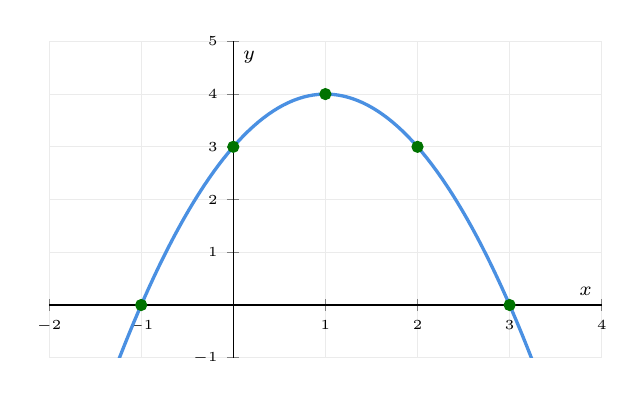
\begin{tikzpicture}\begin{axis}[width=8.6cm,height=5.6cm,axis lines=middle,xlabel={\scriptsize$x$},ylabel={\scriptsize$y$},grid=both,grid style={gray!16},xmin=-2,xmax=4,ymin=-1,ymax=5,xtick distance=1,ytick distance=1,tick label style={font=\tiny},axis line style={-}]
\addplot[exblue,very thick,domain=-1.4:3.4,samples=90]{-x^2+2*x+3};\addplot[only marks,mark=*,mark size=2pt,green!45!black]coordinates{(-1,0)(0,3)(1,4)(2,3)(3,0)};
\end{axis}\end{tikzpicture}\end{center}
\begin{center}\renewcommand{\arraystretch}{1.15}\setlength{\tabcolsep}{2pt}\begin{tabular}{r|>{\centering\arraybackslash}p{0.62cm}>{\centering\arraybackslash}p{0.62cm}>{\centering\arraybackslash}p{0.62cm}>{\centering\arraybackslash}p{0.62cm}>{\centering\arraybackslash}p{0.62cm}>{\centering\arraybackslash}p{0.62cm}>{\centering\arraybackslash}p{0.62cm}>{\centering\arraybackslash}p{0.62cm}>{\centering\arraybackslash}p{0.62cm}>{\centering\arraybackslash}p{0.62cm}}
$x$ & \multicolumn{2}{c}{\colorbox{iagreen}{\makebox[1.12cm]{\strut \color{white}\bfseries $-1$}}} & \multicolumn{2}{c}{\colorbox{iagreen}{\makebox[1.12cm]{\strut \color{white}\bfseries $0$}}} & \multicolumn{2}{c}{\colorbox{iagreen}{\makebox[1.12cm]{\strut \color{white}\bfseries $1$}}} & \multicolumn{2}{c}{\colorbox{iagreen}{\makebox[1.12cm]{\strut \color{white}\bfseries $2$}}} & \multicolumn{2}{c}{\colorbox{iagreen}{\makebox[1.12cm]{\strut \color{white}\bfseries $3$}}} \\[2pt]
$y$ & \multicolumn{2}{c}{\fbox{\makebox[0.94cm]{\strut}}} & \multicolumn{2}{c}{\fbox{\makebox[0.94cm]{\strut}}} & \multicolumn{2}{c}{\fbox{\makebox[0.94cm]{\strut}}} & \multicolumn{2}{c}{\fbox{\makebox[0.94cm]{\strut}}} & \multicolumn{2}{c}{\fbox{\makebox[0.94cm]{\strut}}} \\[2pt]
\textcolor{exblue}{\scriptsize 1st diff} & & \multicolumn{2}{c}{\fbox{\makebox[0.94cm]{\strut}}} & \multicolumn{2}{c}{\fbox{\makebox[0.94cm]{\strut}}} & \multicolumn{2}{c}{\fbox{\makebox[0.94cm]{\strut}}} & \multicolumn{2}{c}{\fbox{\makebox[0.94cm]{\strut}}} & \\[2pt]
\textcolor{qorange}{\scriptsize 2nd diff} & & & \multicolumn{2}{c}{\fbox{\makebox[0.94cm]{\strut}}} & \multicolumn{2}{c}{\fbox{\makebox[0.94cm]{\strut}}} & \multicolumn{2}{c}{\fbox{\makebox[0.94cm]{\strut}}} & & \\
\end{tabular}\end{center}
  \item For $f(x)=x^2-5x+4$, find $f(-1)$ and $f(6)$. Is $(3,-2)$ on the graph of $f$? Show your substitution.
  \item A ball's height is $h=-5t^2+30t$ (metres). Complete the table, find $a$ from the differences, the maximum height, and the time the ball is in the air.
\begin{center}\renewcommand{\arraystretch}{1.15}\setlength{\tabcolsep}{2pt}\begin{tabular}{r|>{\centering\arraybackslash}p{0.62cm}>{\centering\arraybackslash}p{0.62cm}>{\centering\arraybackslash}p{0.62cm}>{\centering\arraybackslash}p{0.62cm}>{\centering\arraybackslash}p{0.62cm}>{\centering\arraybackslash}p{0.62cm}>{\centering\arraybackslash}p{0.62cm}>{\centering\arraybackslash}p{0.62cm}>{\centering\arraybackslash}p{0.62cm}>{\centering\arraybackslash}p{0.62cm}>{\centering\arraybackslash}p{0.62cm}>{\centering\arraybackslash}p{0.62cm}>{\centering\arraybackslash}p{0.62cm}>{\centering\arraybackslash}p{0.62cm}}
$x$ & \multicolumn{2}{c}{\colorbox{iagreen}{\makebox[1.12cm]{\strut \color{white}\bfseries $0$}}} & \multicolumn{2}{c}{\colorbox{iagreen}{\makebox[1.12cm]{\strut \color{white}\bfseries $1$}}} & \multicolumn{2}{c}{\colorbox{iagreen}{\makebox[1.12cm]{\strut \color{white}\bfseries $2$}}} & \multicolumn{2}{c}{\colorbox{iagreen}{\makebox[1.12cm]{\strut \color{white}\bfseries $3$}}} & \multicolumn{2}{c}{\colorbox{iagreen}{\makebox[1.12cm]{\strut \color{white}\bfseries $4$}}} & \multicolumn{2}{c}{\colorbox{iagreen}{\makebox[1.12cm]{\strut \color{white}\bfseries $5$}}} & \multicolumn{2}{c}{\colorbox{iagreen}{\makebox[1.12cm]{\strut \color{white}\bfseries $6$}}} \\[2pt]
$h$ & \multicolumn{2}{c}{\fbox{\makebox[0.94cm]{\strut}}} & \multicolumn{2}{c}{\fbox{\makebox[0.94cm]{\strut}}} & \multicolumn{2}{c}{\fbox{\makebox[0.94cm]{\strut}}} & \multicolumn{2}{c}{\fbox{\makebox[0.94cm]{\strut}}} & \multicolumn{2}{c}{\fbox{\makebox[0.94cm]{\strut}}} & \multicolumn{2}{c}{\fbox{\makebox[0.94cm]{\strut}}} & \multicolumn{2}{c}{\fbox{\makebox[0.94cm]{\strut}}} \\[2pt]
\textcolor{exblue}{\scriptsize 1st diff} & & \multicolumn{2}{c}{\fbox{\makebox[0.94cm]{\strut}}} & \multicolumn{2}{c}{\fbox{\makebox[0.94cm]{\strut}}} & \multicolumn{2}{c}{\fbox{\makebox[0.94cm]{\strut}}} & \multicolumn{2}{c}{\fbox{\makebox[0.94cm]{\strut}}} & \multicolumn{2}{c}{\fbox{\makebox[0.94cm]{\strut}}} & \multicolumn{2}{c}{\fbox{\makebox[0.94cm]{\strut}}} & \\[2pt]
\textcolor{qorange}{\scriptsize 2nd diff} & & & \multicolumn{2}{c}{\fbox{\makebox[0.94cm]{\strut}}} & \multicolumn{2}{c}{\fbox{\makebox[0.94cm]{\strut}}} & \multicolumn{2}{c}{\fbox{\makebox[0.94cm]{\strut}}} & \multicolumn{2}{c}{\fbox{\makebox[0.94cm]{\strut}}} & \multicolumn{2}{c}{\fbox{\makebox[0.94cm]{\strut}}} & & \\
\end{tabular}\end{center}
  \item One value in this table is wrong. Find it and correct it.
\begin{center}\renewcommand{\arraystretch}{1.15}\setlength{\tabcolsep}{2pt}\begin{tabular}{r|>{\centering\arraybackslash}p{0.62cm}>{\centering\arraybackslash}p{0.62cm}>{\centering\arraybackslash}p{0.62cm}>{\centering\arraybackslash}p{0.62cm}>{\centering\arraybackslash}p{0.62cm}>{\centering\arraybackslash}p{0.62cm}>{\centering\arraybackslash}p{0.62cm}>{\centering\arraybackslash}p{0.62cm}>{\centering\arraybackslash}p{0.62cm}>{\centering\arraybackslash}p{0.62cm}}
$x$ & \multicolumn{2}{c}{\colorbox{iagreen}{\makebox[1.12cm]{\strut \color{white}\bfseries $0$}}} & \multicolumn{2}{c}{\colorbox{iagreen}{\makebox[1.12cm]{\strut \color{white}\bfseries $1$}}} & \multicolumn{2}{c}{\colorbox{iagreen}{\makebox[1.12cm]{\strut \color{white}\bfseries $2$}}} & \multicolumn{2}{c}{\colorbox{iagreen}{\makebox[1.12cm]{\strut \color{white}\bfseries $3$}}} & \multicolumn{2}{c}{\colorbox{iagreen}{\makebox[1.12cm]{\strut \color{white}\bfseries $4$}}} \\[2pt]
$y$ & \multicolumn{2}{c}{\colorbox{keybg}{\makebox[1.12cm]{\strut $1$}}} & \multicolumn{2}{c}{\colorbox{keybg}{\makebox[1.12cm]{\strut $4$}}} & \multicolumn{2}{c}{\colorbox{keybg}{\makebox[1.12cm]{\strut $9$}}} & \multicolumn{2}{c}{\colorbox{keybg}{\makebox[1.12cm]{\strut $17$}}} & \multicolumn{2}{c}{\colorbox{keybg}{\makebox[1.12cm]{\strut $25$}}} \\[2pt]
\textcolor{exblue}{\scriptsize 1st diff} & & \multicolumn{2}{c}{\colorbox{exbg}{\makebox[1.12cm]{\strut \textcolor{exblue}{$+3$}}}} & \multicolumn{2}{c}{\colorbox{exbg}{\makebox[1.12cm]{\strut \textcolor{exblue}{$+5$}}}} & \multicolumn{2}{c}{\colorbox{exbg}{\makebox[1.12cm]{\strut \textcolor{exblue}{$+8$}}}} & \multicolumn{2}{c}{\colorbox{exbg}{\makebox[1.12cm]{\strut \textcolor{exblue}{$+8$}}}} & \\[2pt]
\textcolor{qorange}{\scriptsize 2nd diff} & & & \multicolumn{2}{c}{\colorbox{qbg}{\makebox[1.12cm]{\strut \textcolor{qorange!70!black}{$+2$}}}} & \multicolumn{2}{c}{\colorbox{qbg}{\makebox[1.12cm]{\strut \textcolor{qorange!70!black}{$+3$}}}} & \multicolumn{2}{c}{\colorbox{qbg}{\makebox[1.12cm]{\strut \textcolor{qorange!70!black}{$+0$}}}} & & \\
\end{tabular}\end{center}
  \item Show that for $y=ax^2+bx+c$ and $x=0,1,2$, the second difference is $2a$.
  \item A quadratic relation passes through $(0,-5)$, $(1,-2)$ and $(2,5)$. Find $y$ when $x=10$, and say whether $(3,16)$ is on the graph.
\end{enumerate}
\end{multicols}
\end{recapbox}

\begin{keybox}
\begin{multicols}{2}
\small
\begin{enumerate}[leftmargin=*,itemsep=3pt]
  \item A: 1st $3,5,7,9$; 2nd $2,2,2$ --- quadratic. B: 1st $4,4,4,4$ --- linear.
  \item $y$: $5,-1,-3,-1,5$; 1st: $-6,-2,2,6$; 2nd: $4,4,4$ (so $a=2$).
  \item $y$-values $4,2,2,?,8,14$; 1st differences $-2,0,2,4,6$: the missing value is $2+2=4$.
  \item $A$ and $B$ are on the graph. $y(4)=-1$, so $C$ should be $(4,-1)$; $y(5)=2$, so $D$ should be $(5,2)$.
  \item 2nd difference $6$, so $a=3$; $c=1$; at $x=1$: $3+b+1=2$, so $b=-2$. $y=3x^2-2x+1$.
  \item 2nd difference $-2$, so $a=-1$ (opens down). Vertex $(3,5)$.
  \item 2nd difference $8=2a(2)^2$, so $a=1$; $c=1$; at $x=2$: $4+2b+1=5$, so $b=0$. $y=x^2+1$.
  \item Table $y$: $0,3,4,3,0$; 1st: $3,1,-1,-3$; 2nd: $-2,-2,-2$; $a=-1$.
  \item $f(-1)=1+5+4=10$; $f(6)=36-30+4=10$; $f(3)=9-15+4=-2$, so $(3,-2)$ \textbf{is} on the graph.
  \item $h$: $0,25,40,45,40,25,0$; 2nd difference $-10$, so $a=-5$; maximum $45$ m at $t=3$ s; in the air $6$ s.
  \item 2nd differences $2,3,0$ are not constant. The value $17$ should be $16$ (then 1st differences $3,5,7,9$).
  \item $y(0)=c$, $y(1)=a+b+c$, $y(2)=4a+2b+c$. 1st: $a+b$ and $3a+b$. 2nd: $(3a+b)-(a+b)=2a$.
  \item 2nd difference $4$, so $a=2$; $c=-5$; $2+b-5=-2$ gives $b=1$. $y=2x^2+x-5$; $y(10)=205$. At $x=3$: $18+3-5=16$, so $(3,16)$ is on the graph.
\end{enumerate}
\end{multicols}
\end{keybox}

\end{document}
